\chapter{Parameter Values Distributions in Terms of Quality}\label{appendix:Distributions3}
\begin{figure}
	\centering
	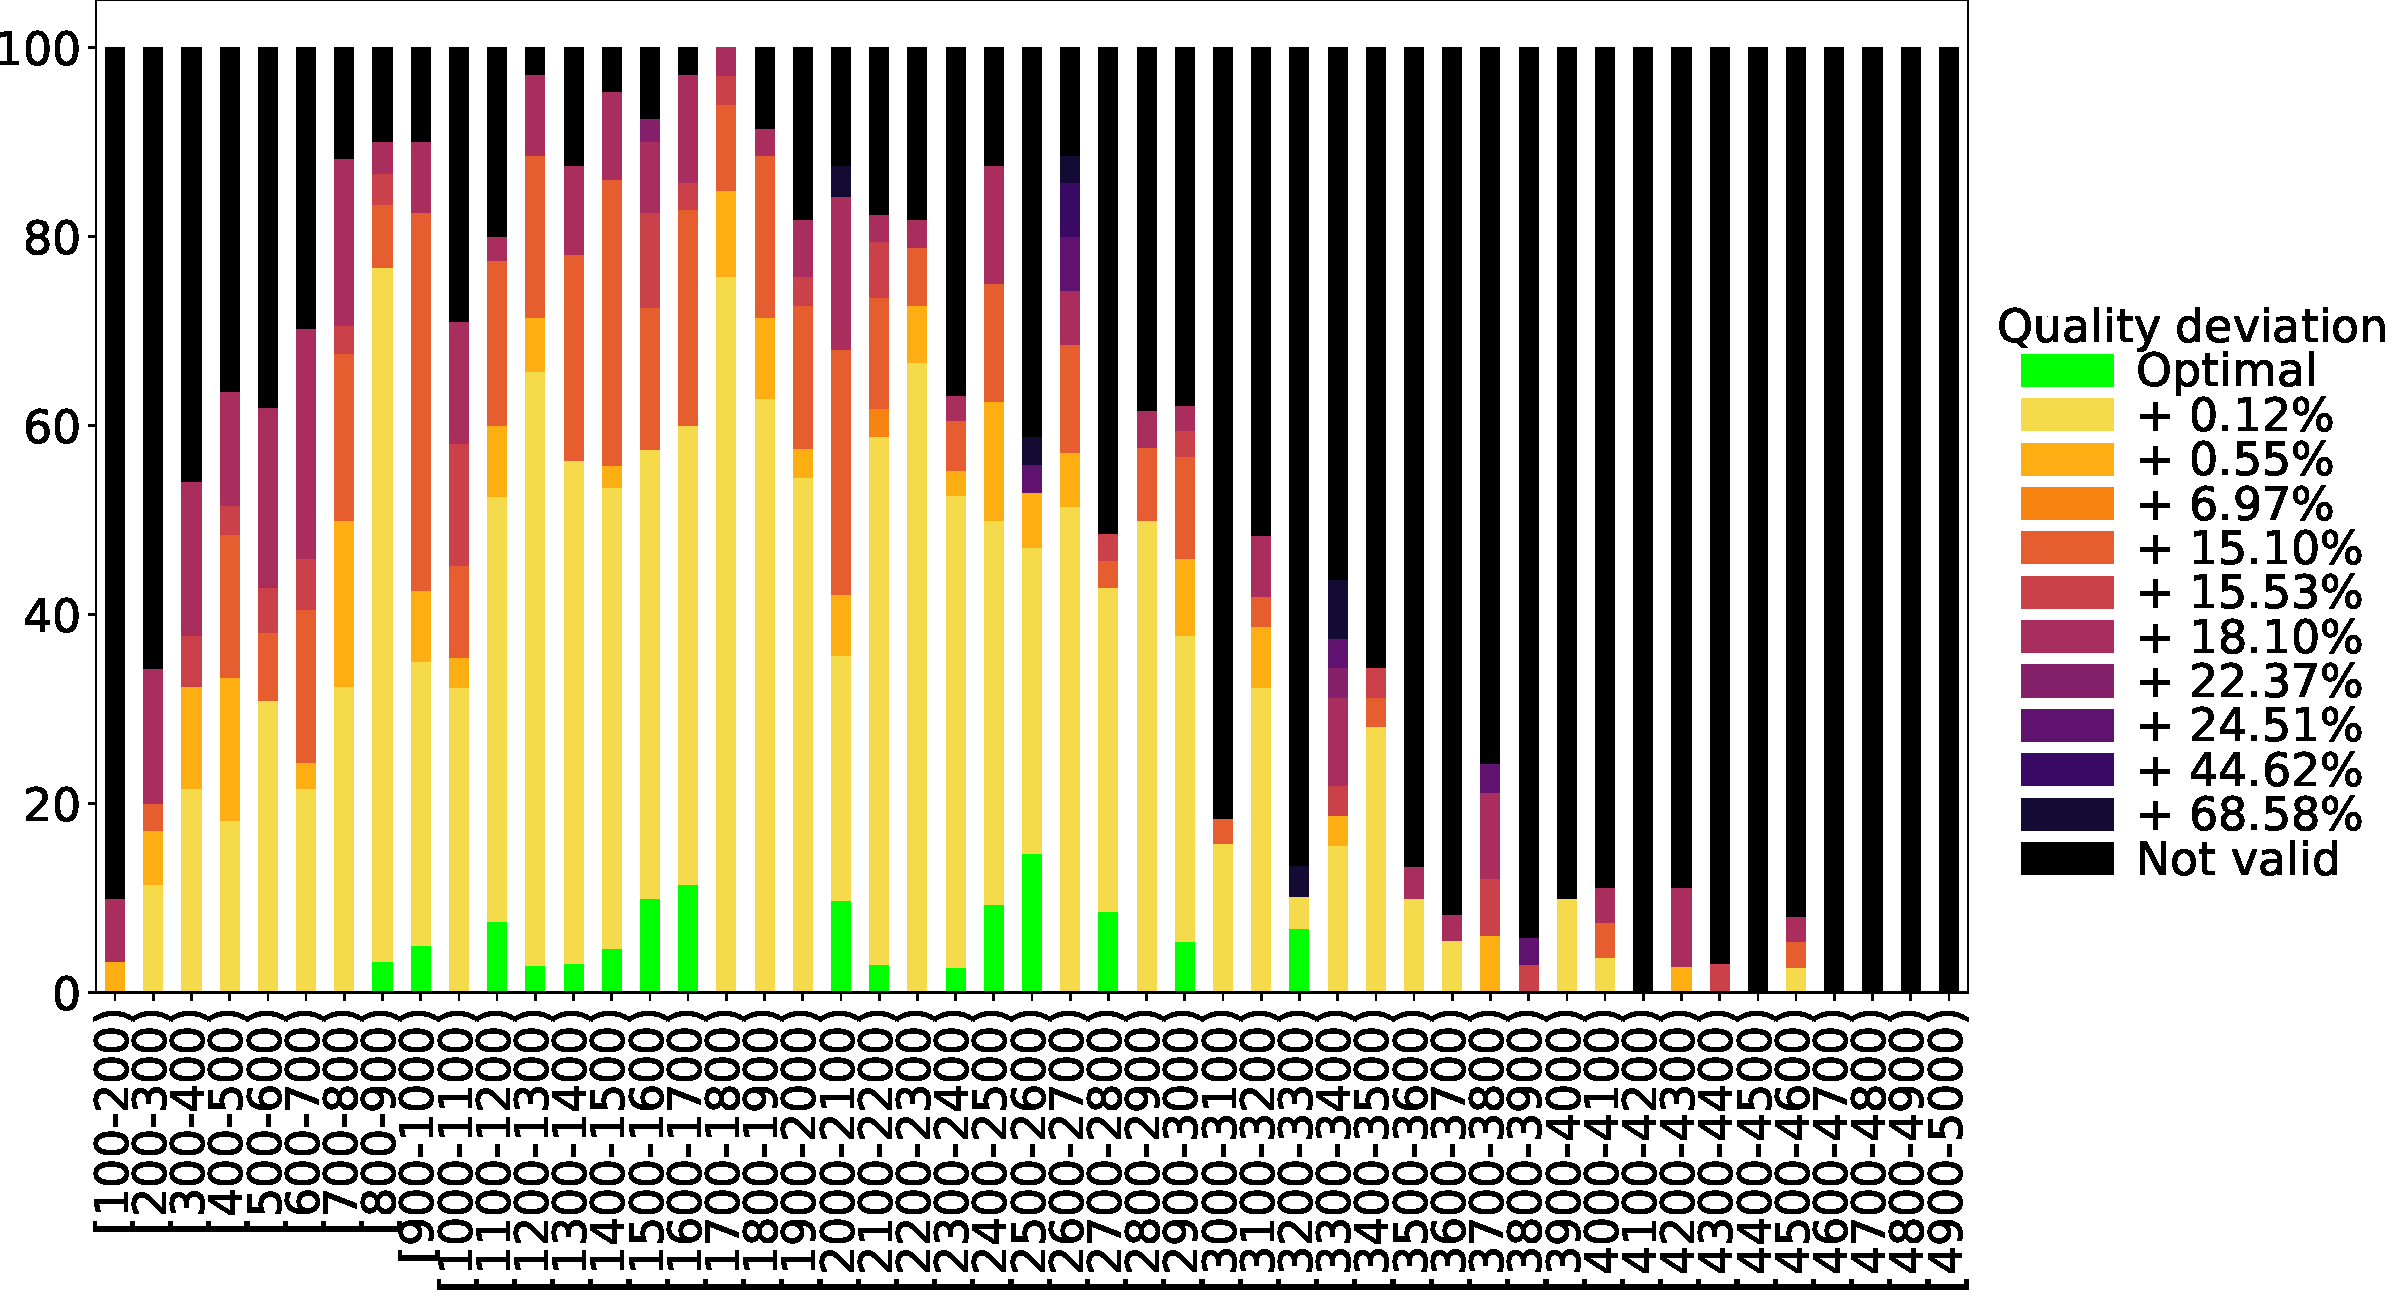
\includegraphics[width=\textwidth]{images/DistrObj/populationSize.pdf}
	\caption[populationSize parameter values distribution for smaller problem]{populationSize parameter values distribution for smaller problem}
	\label{fig:populationSize_Obj}
\end{figure}
\begin{figure}
	\centering
	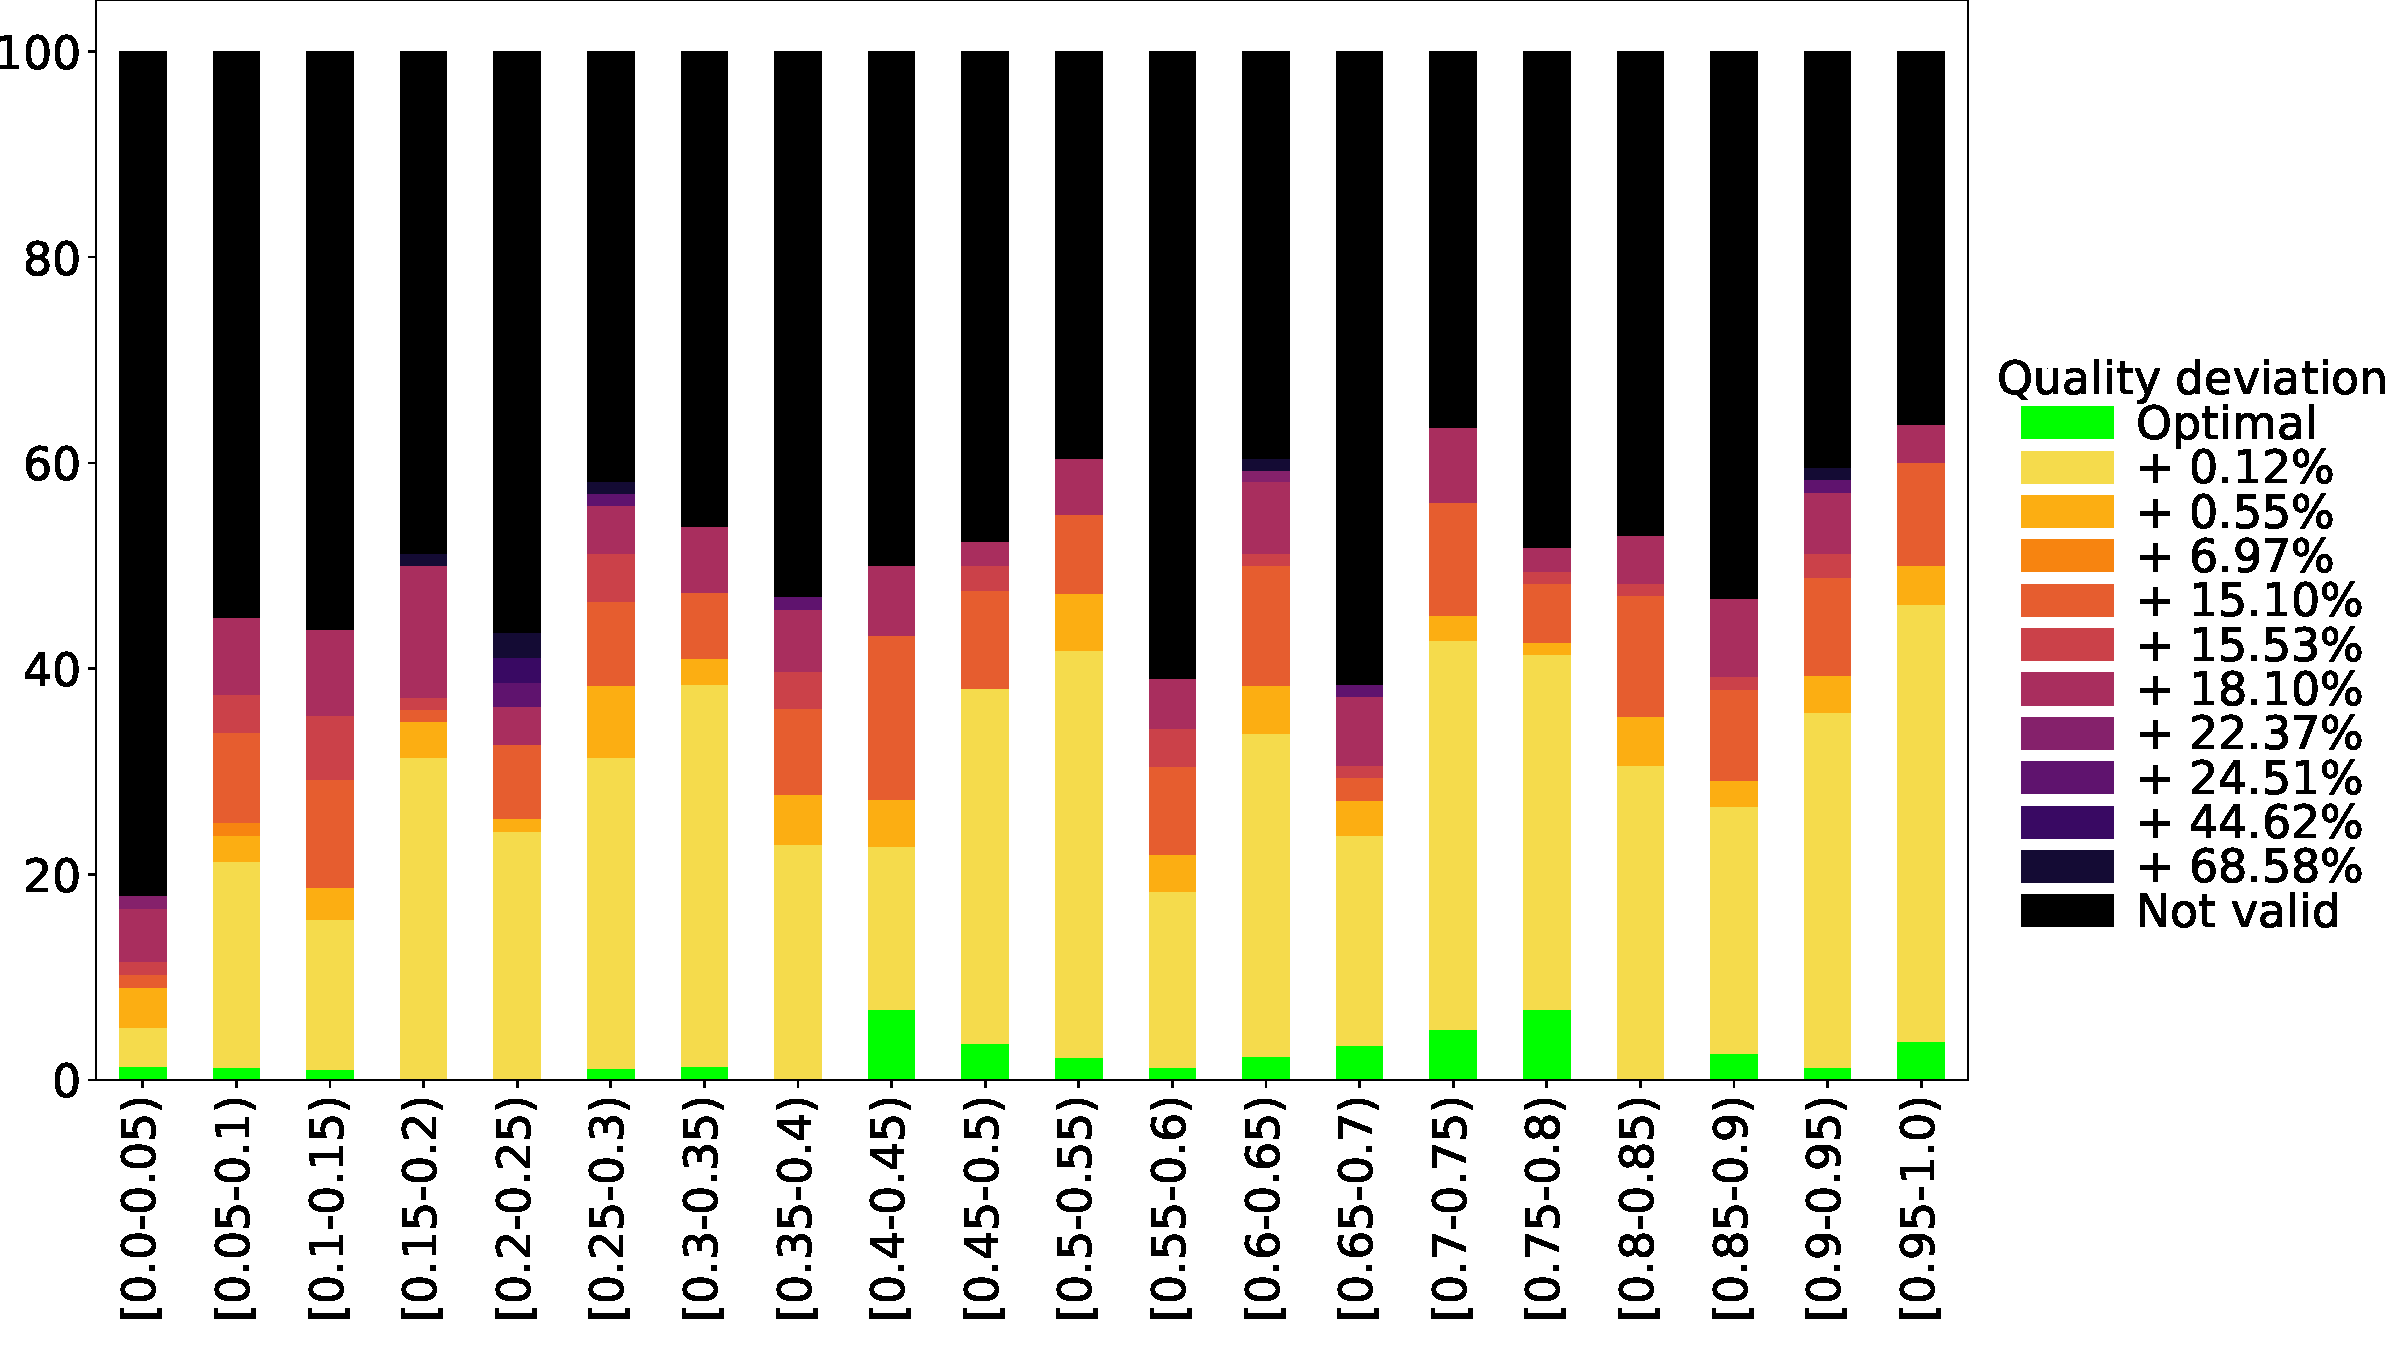
\includegraphics[width=\textwidth]{images/DistrObj/lambda.pdf}
	\caption[lambda parameter values distribution for smaller problem]{lambda parameter values distribution for smaller problem}
	\label{fig:lambda_Obj}
\end{figure}
\begin{figure}
	\centering
	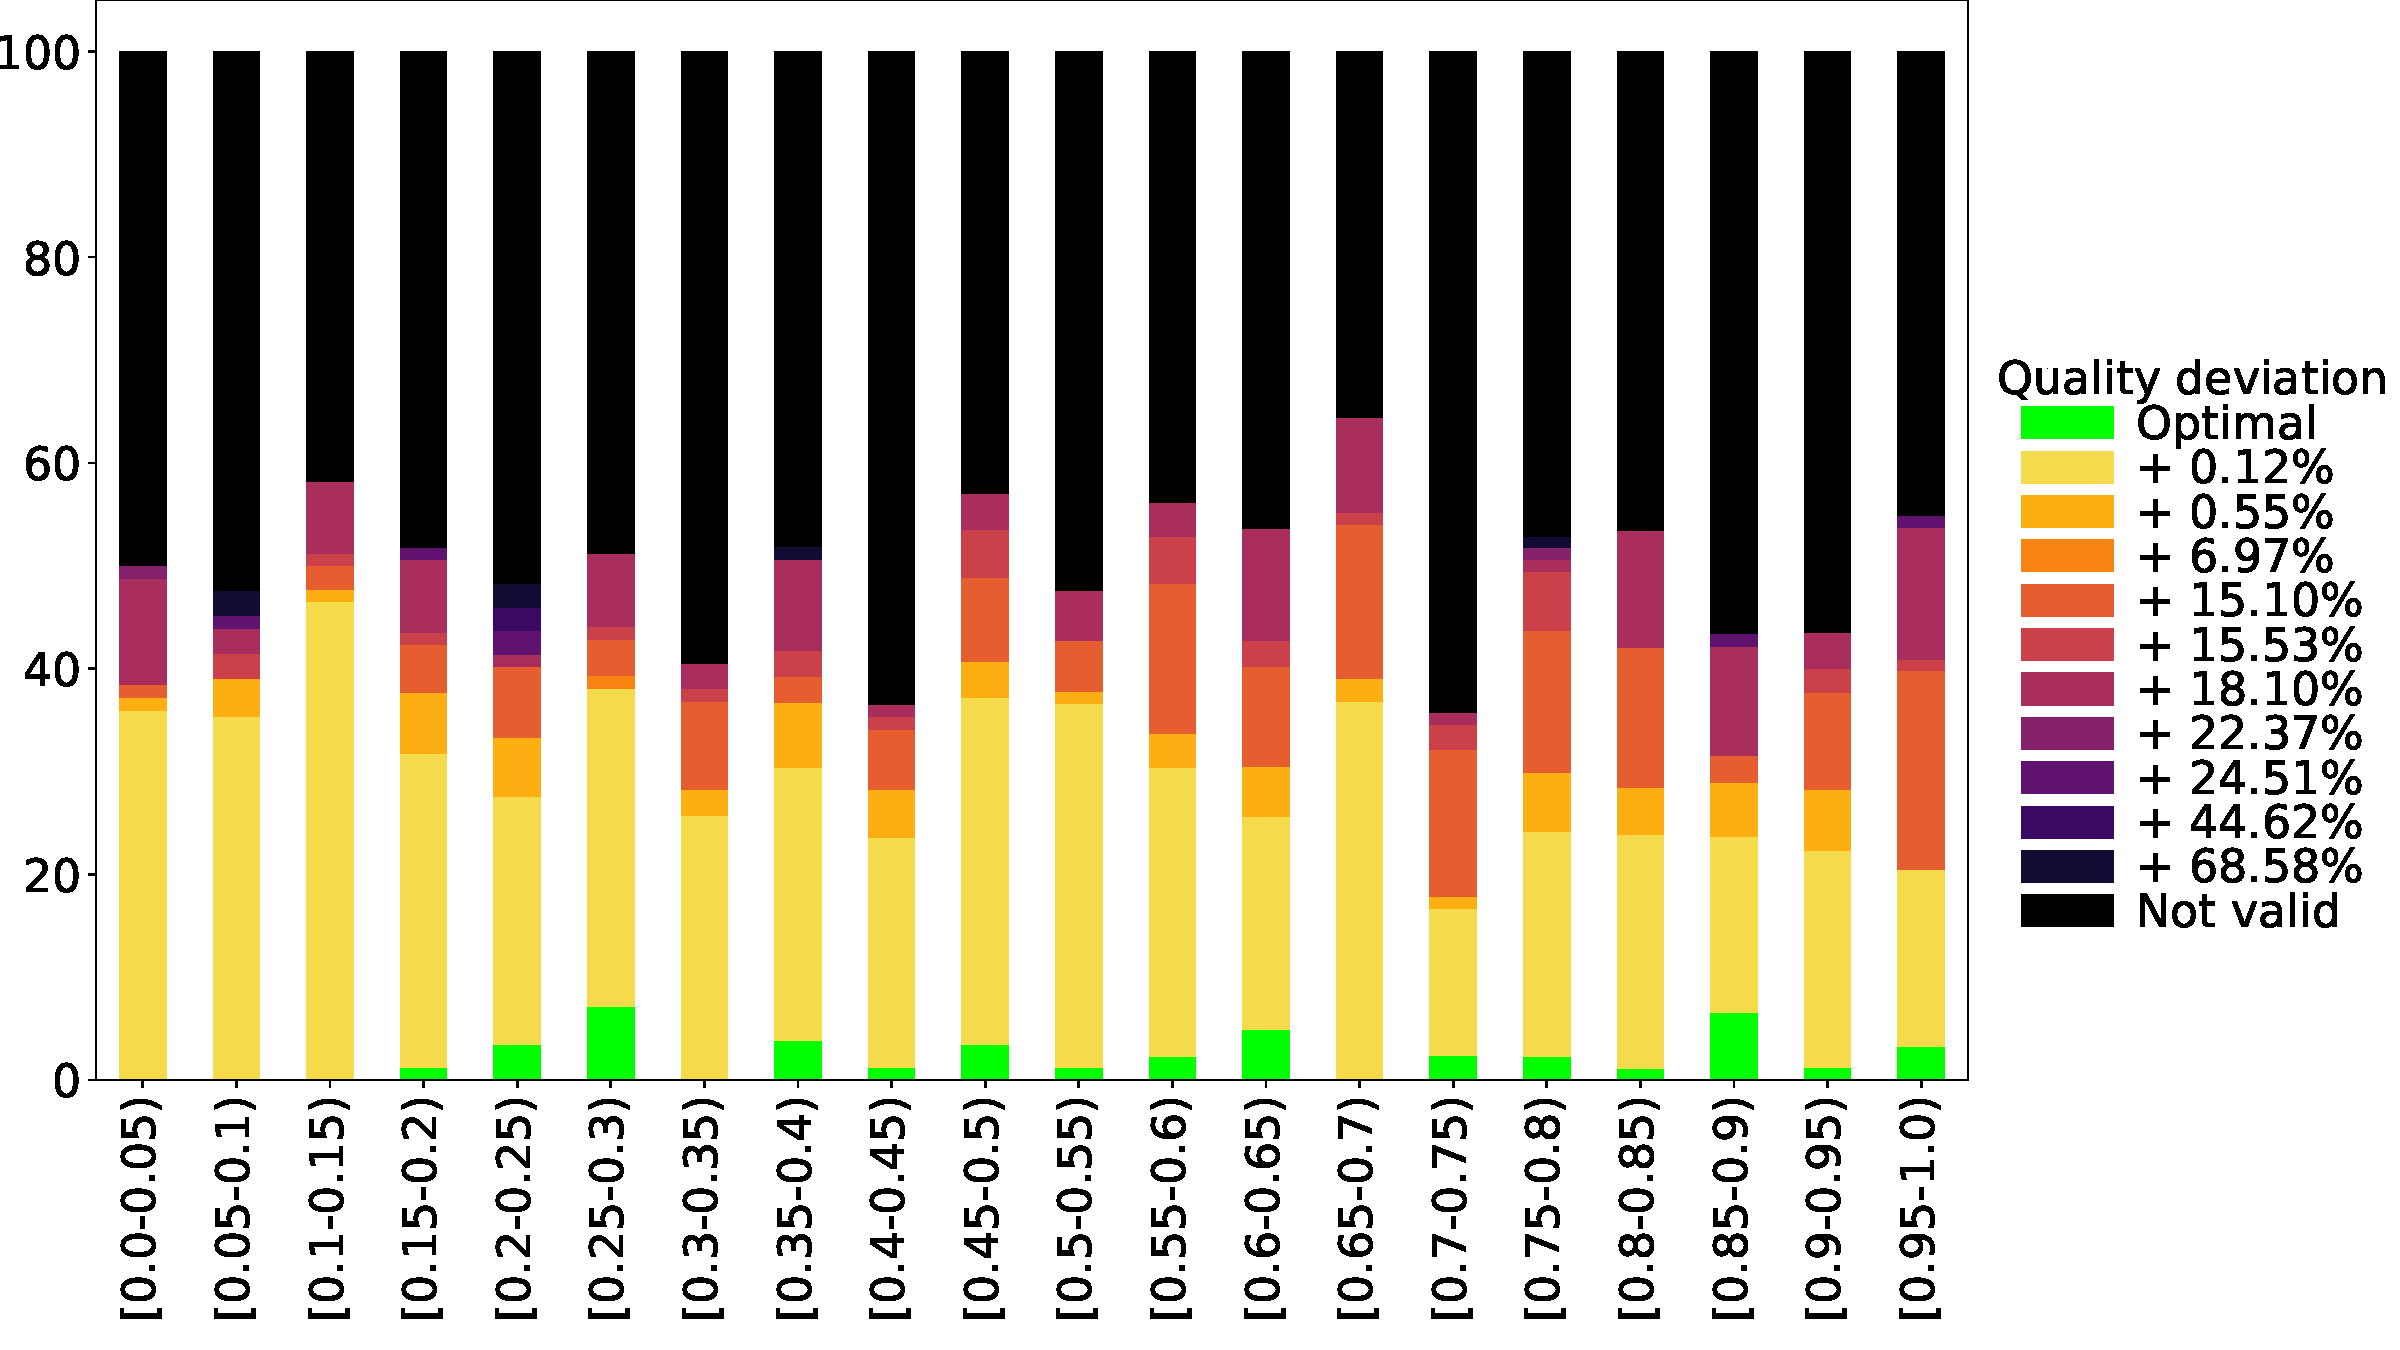
\includegraphics[width=\textwidth]{images/DistrObj/crossoverRate.pdf}
	\caption[crossoverRate parameter values distribution for smaller problem]{crossoverRate parameter values distribution for smaller problem}  
	\label{fig:crossoverRate_Obj}
\end{figure}
\begin{figure}
	\centering
	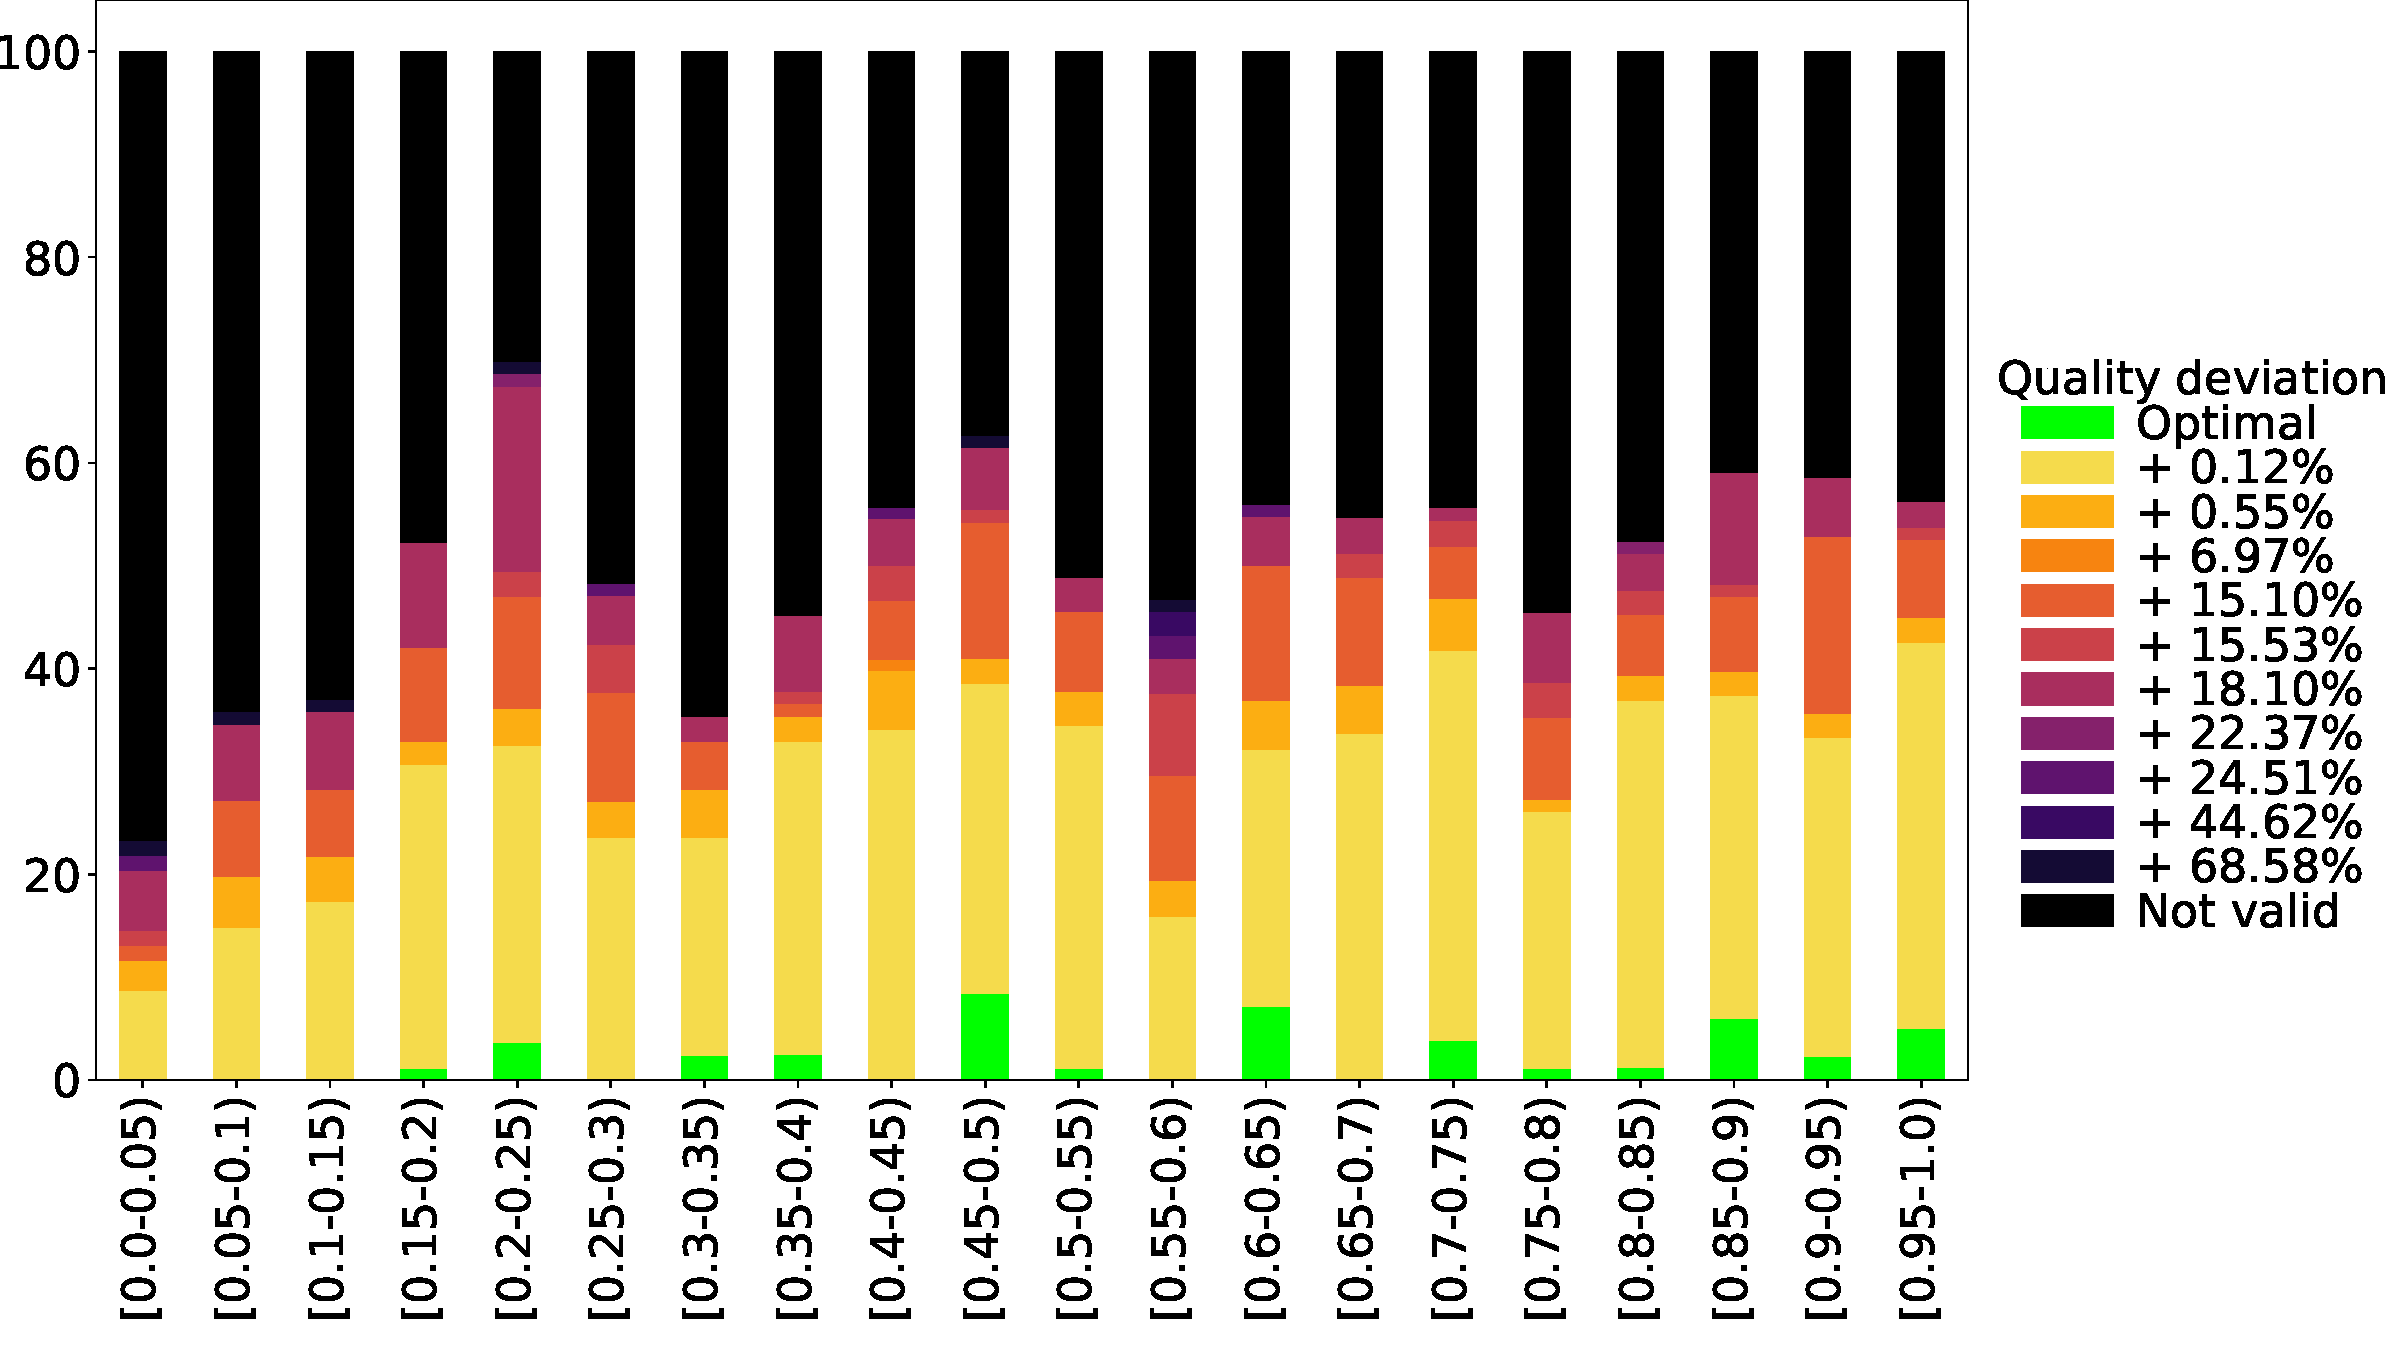
\includegraphics[width=\textwidth]{images/DistrObj/mu.pdf}
	\caption[mu parameter values distribution for smaller problem]{mu parameter values distribution for smaller problem}
	\label{fig:mu_Obj}
\end{figure}
\begin{figure}
	\centering
	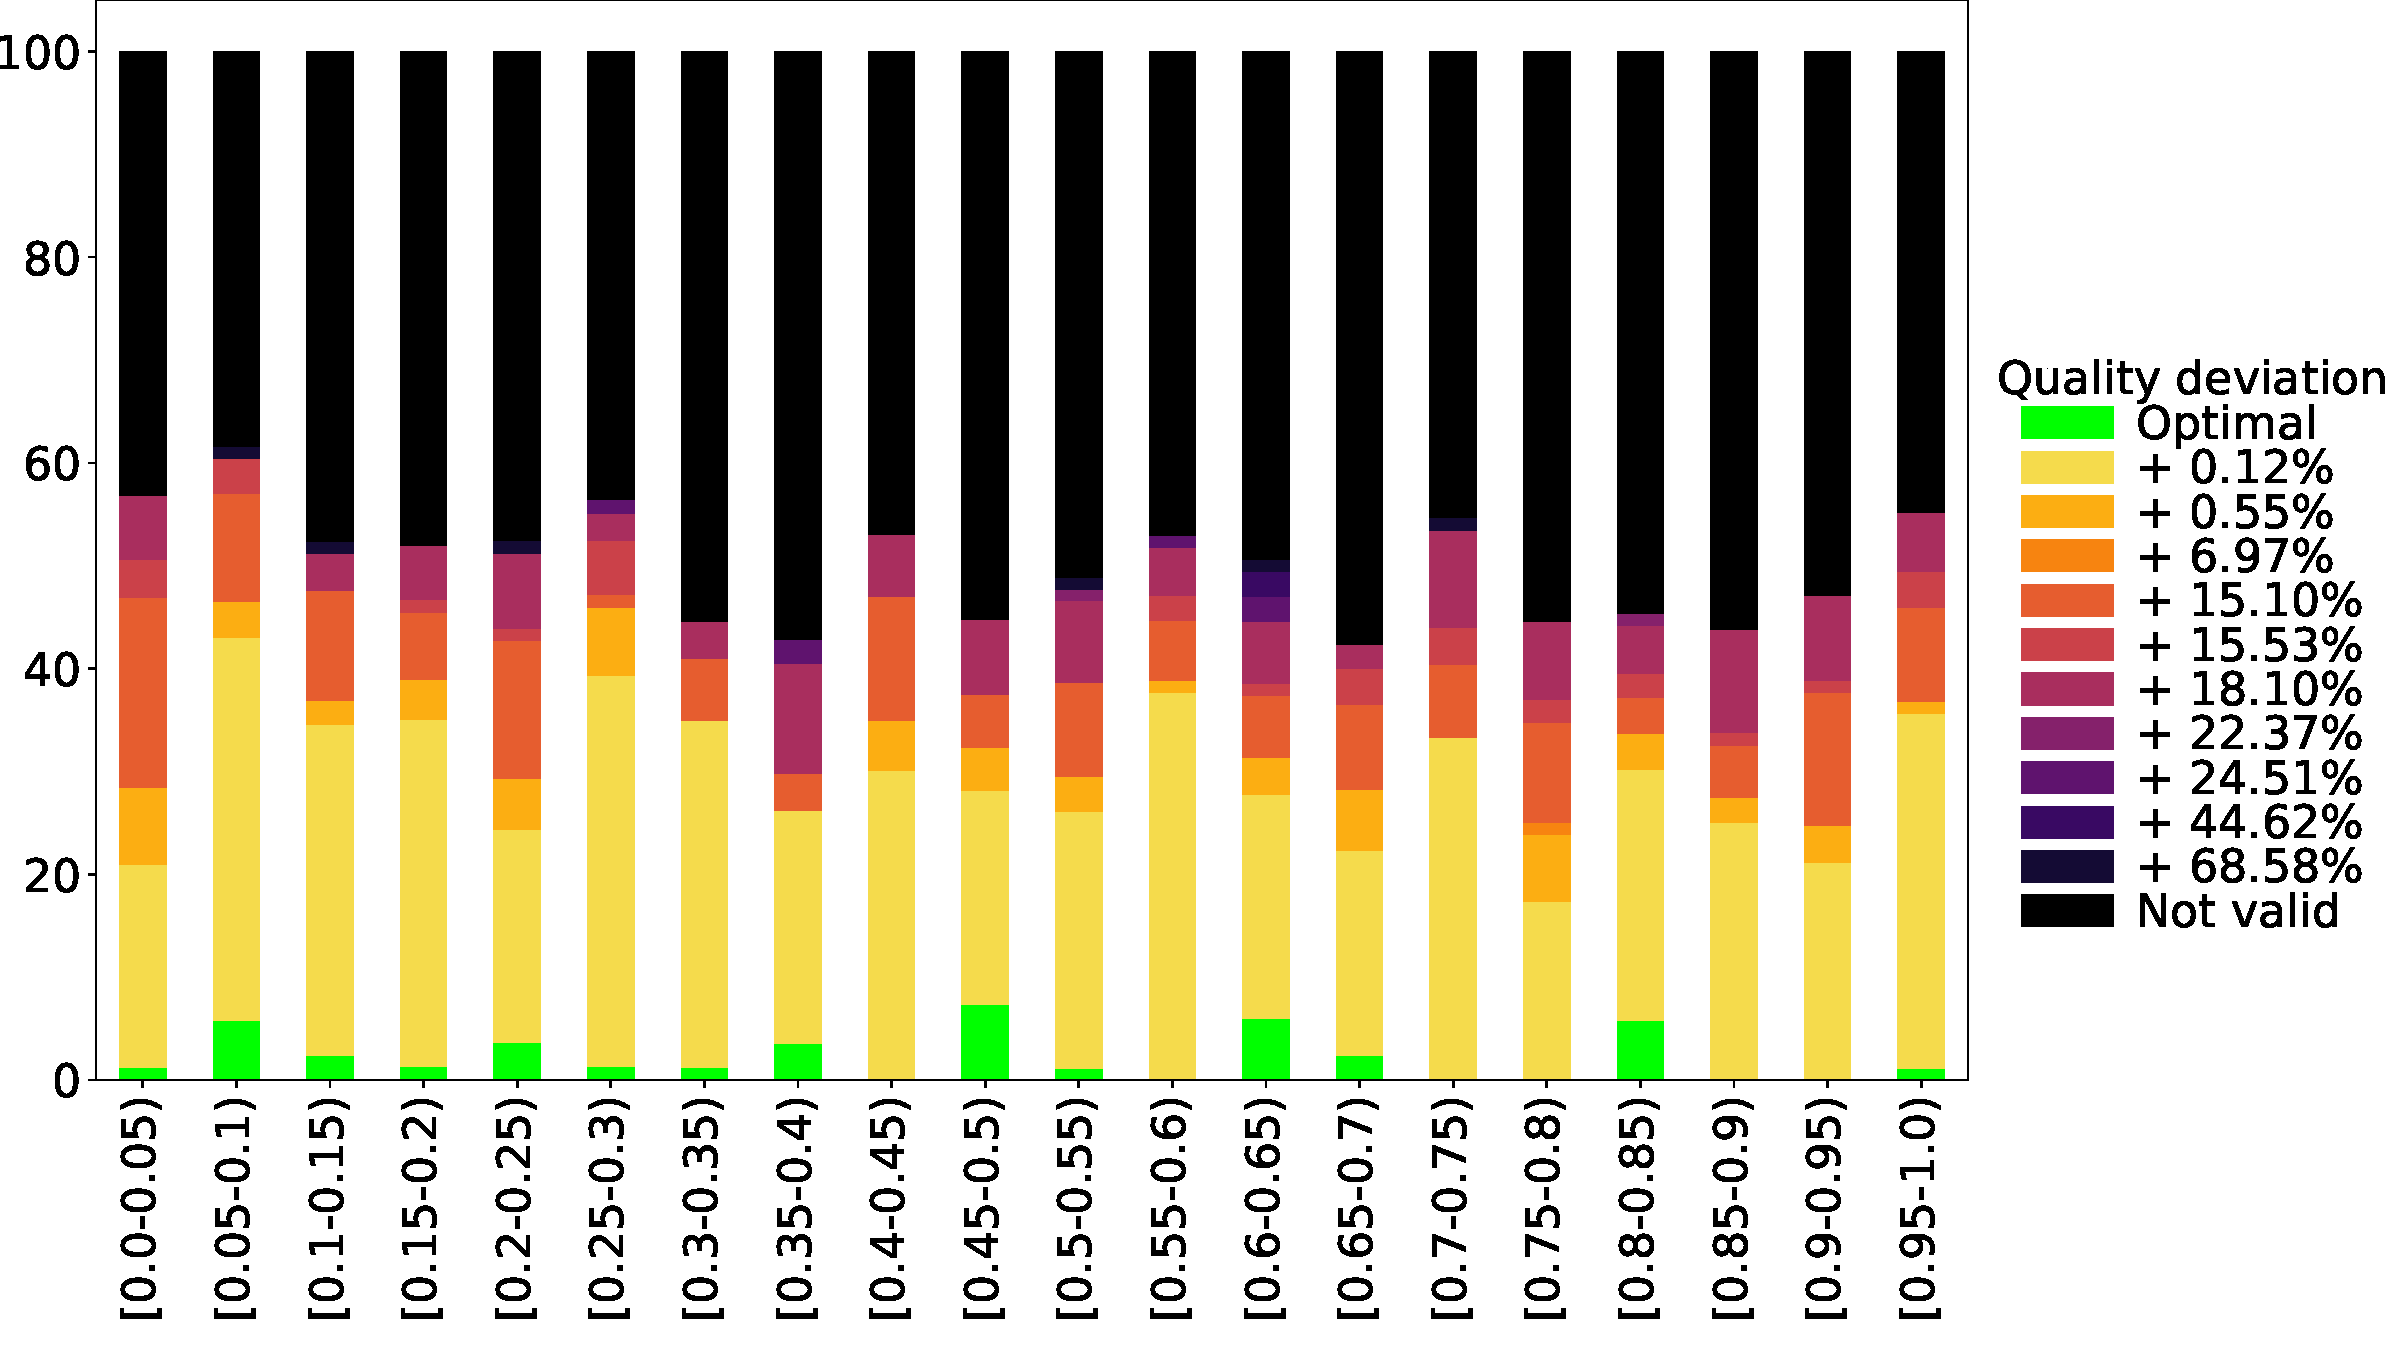
\includegraphics[width=\textwidth]{images/DistrObj/mutationRate.pdf}
	\caption[mutationRate parameter values distribution for smaller problem]{mutationRate parameter values distribution for smaller problem}
	\label{fig:mutationRate_Obj}
\end{figure}
\begin{figure}
	\centering
	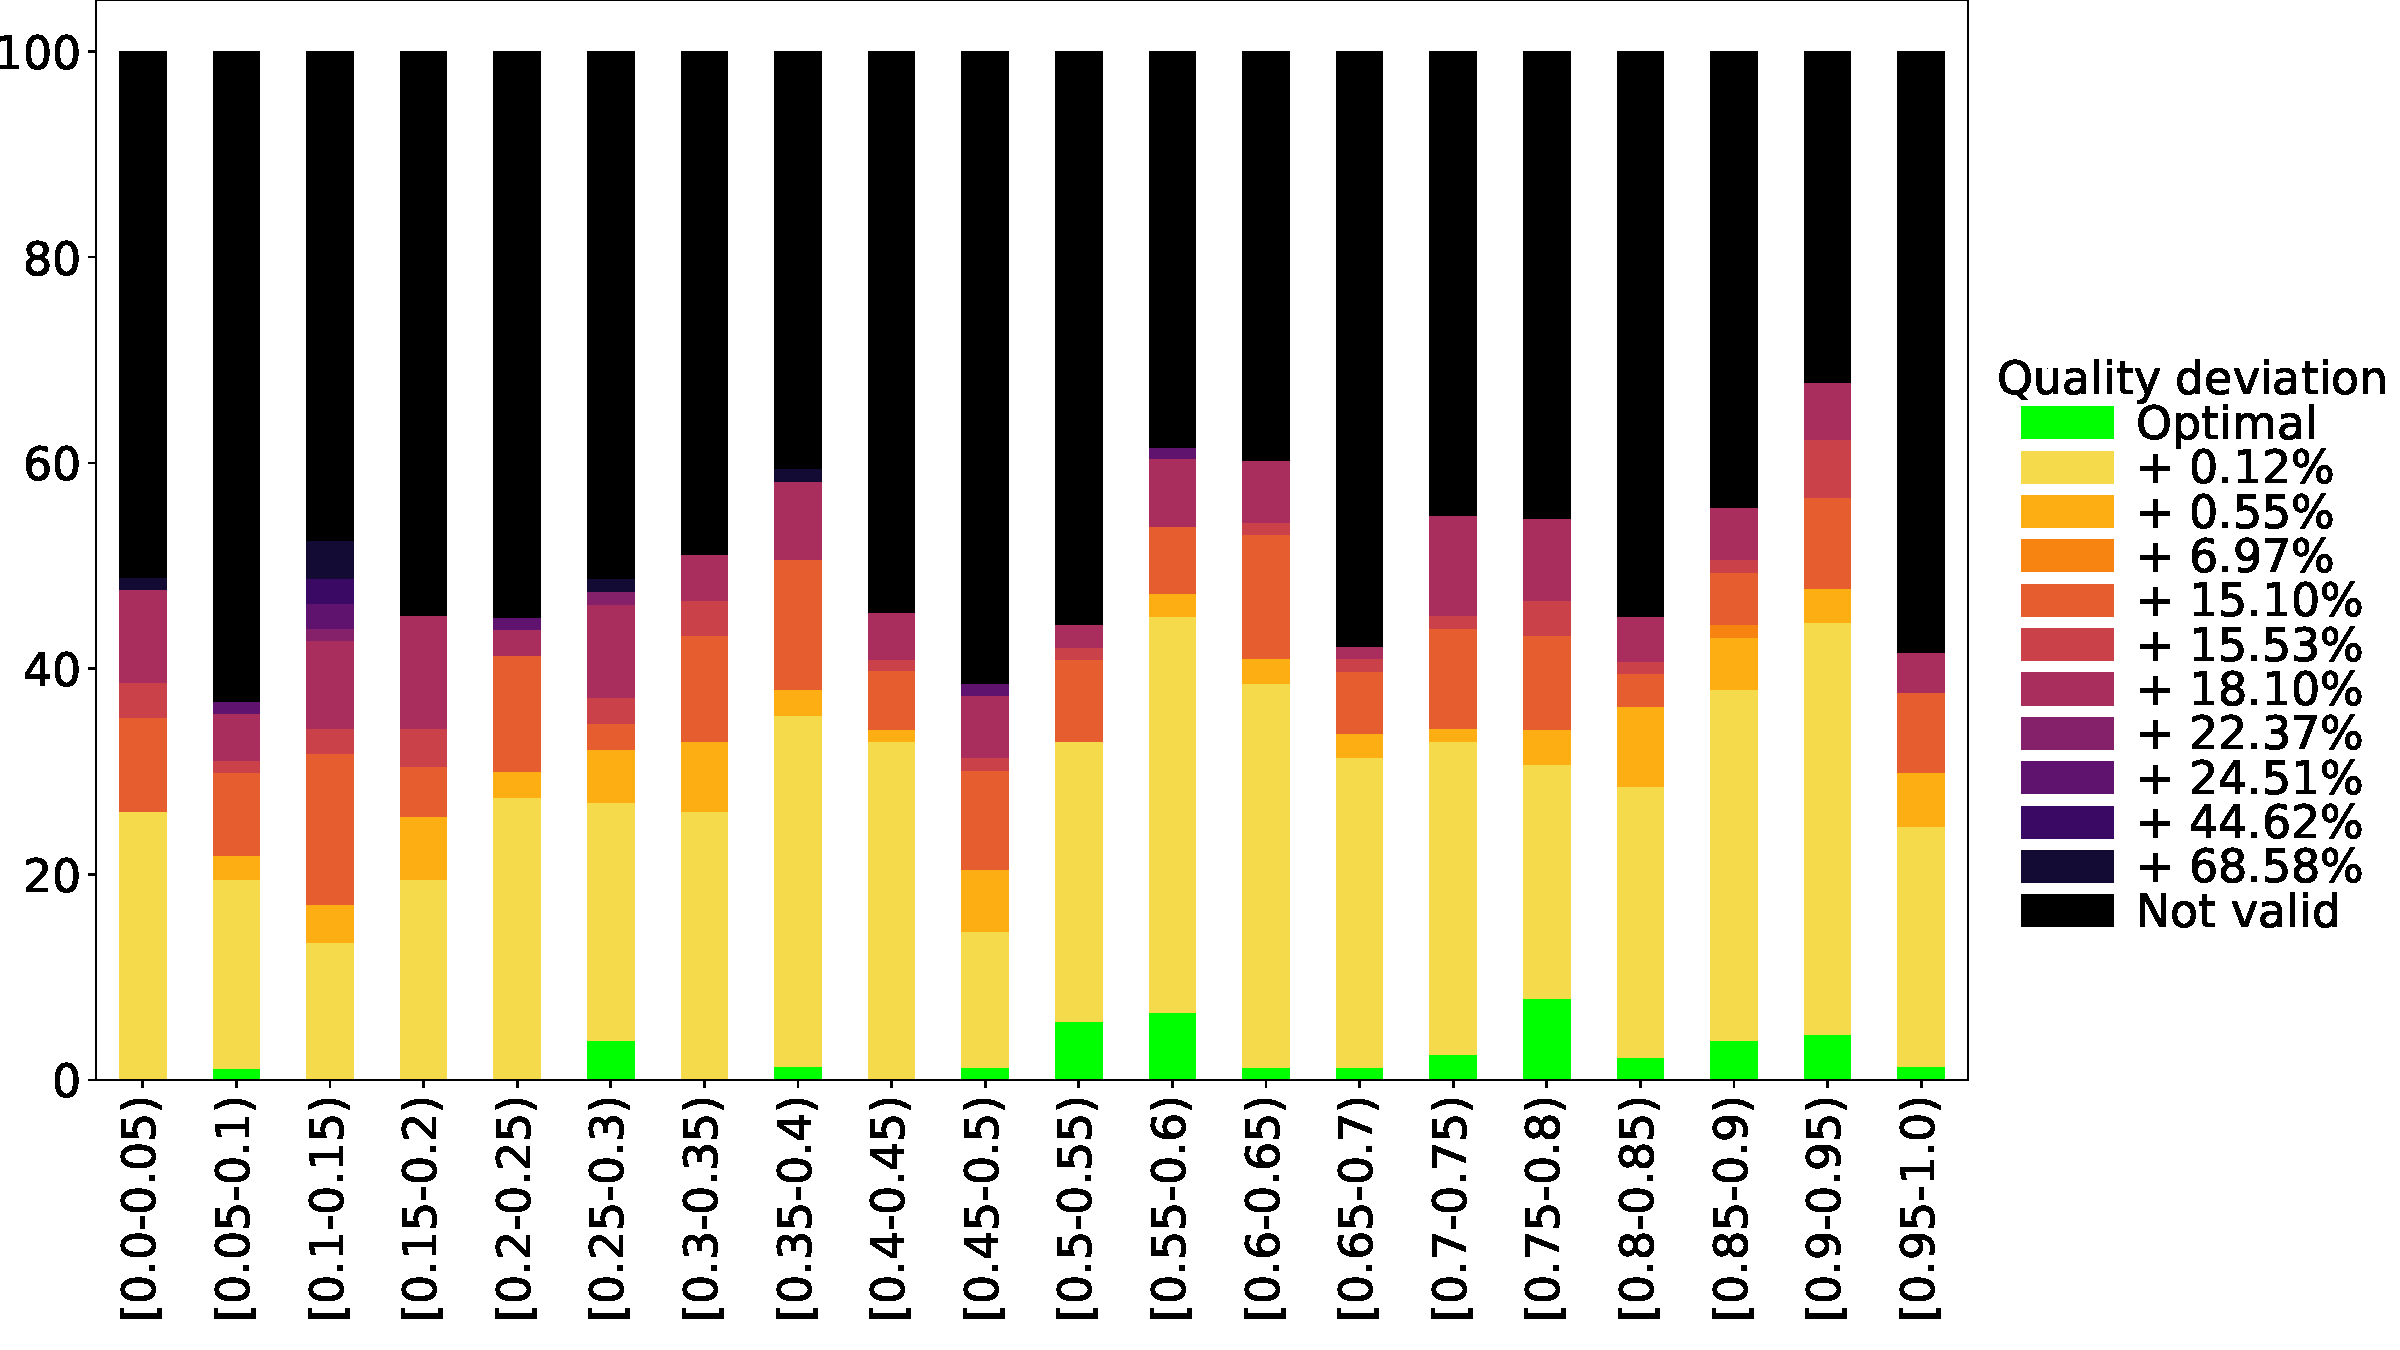
\includegraphics[width=\textwidth]{images/DistrObj/resourcesMutationProbability.pdf}
	\caption[resourcesMutationProbability parameter values distribution for smaller problem]{resourcesMutationProbability parameter values distribution for smaller problem}
	\label{fig:resourcesMutationProbability_Obj}
\end{figure}
\begin{figure}
	\centering
	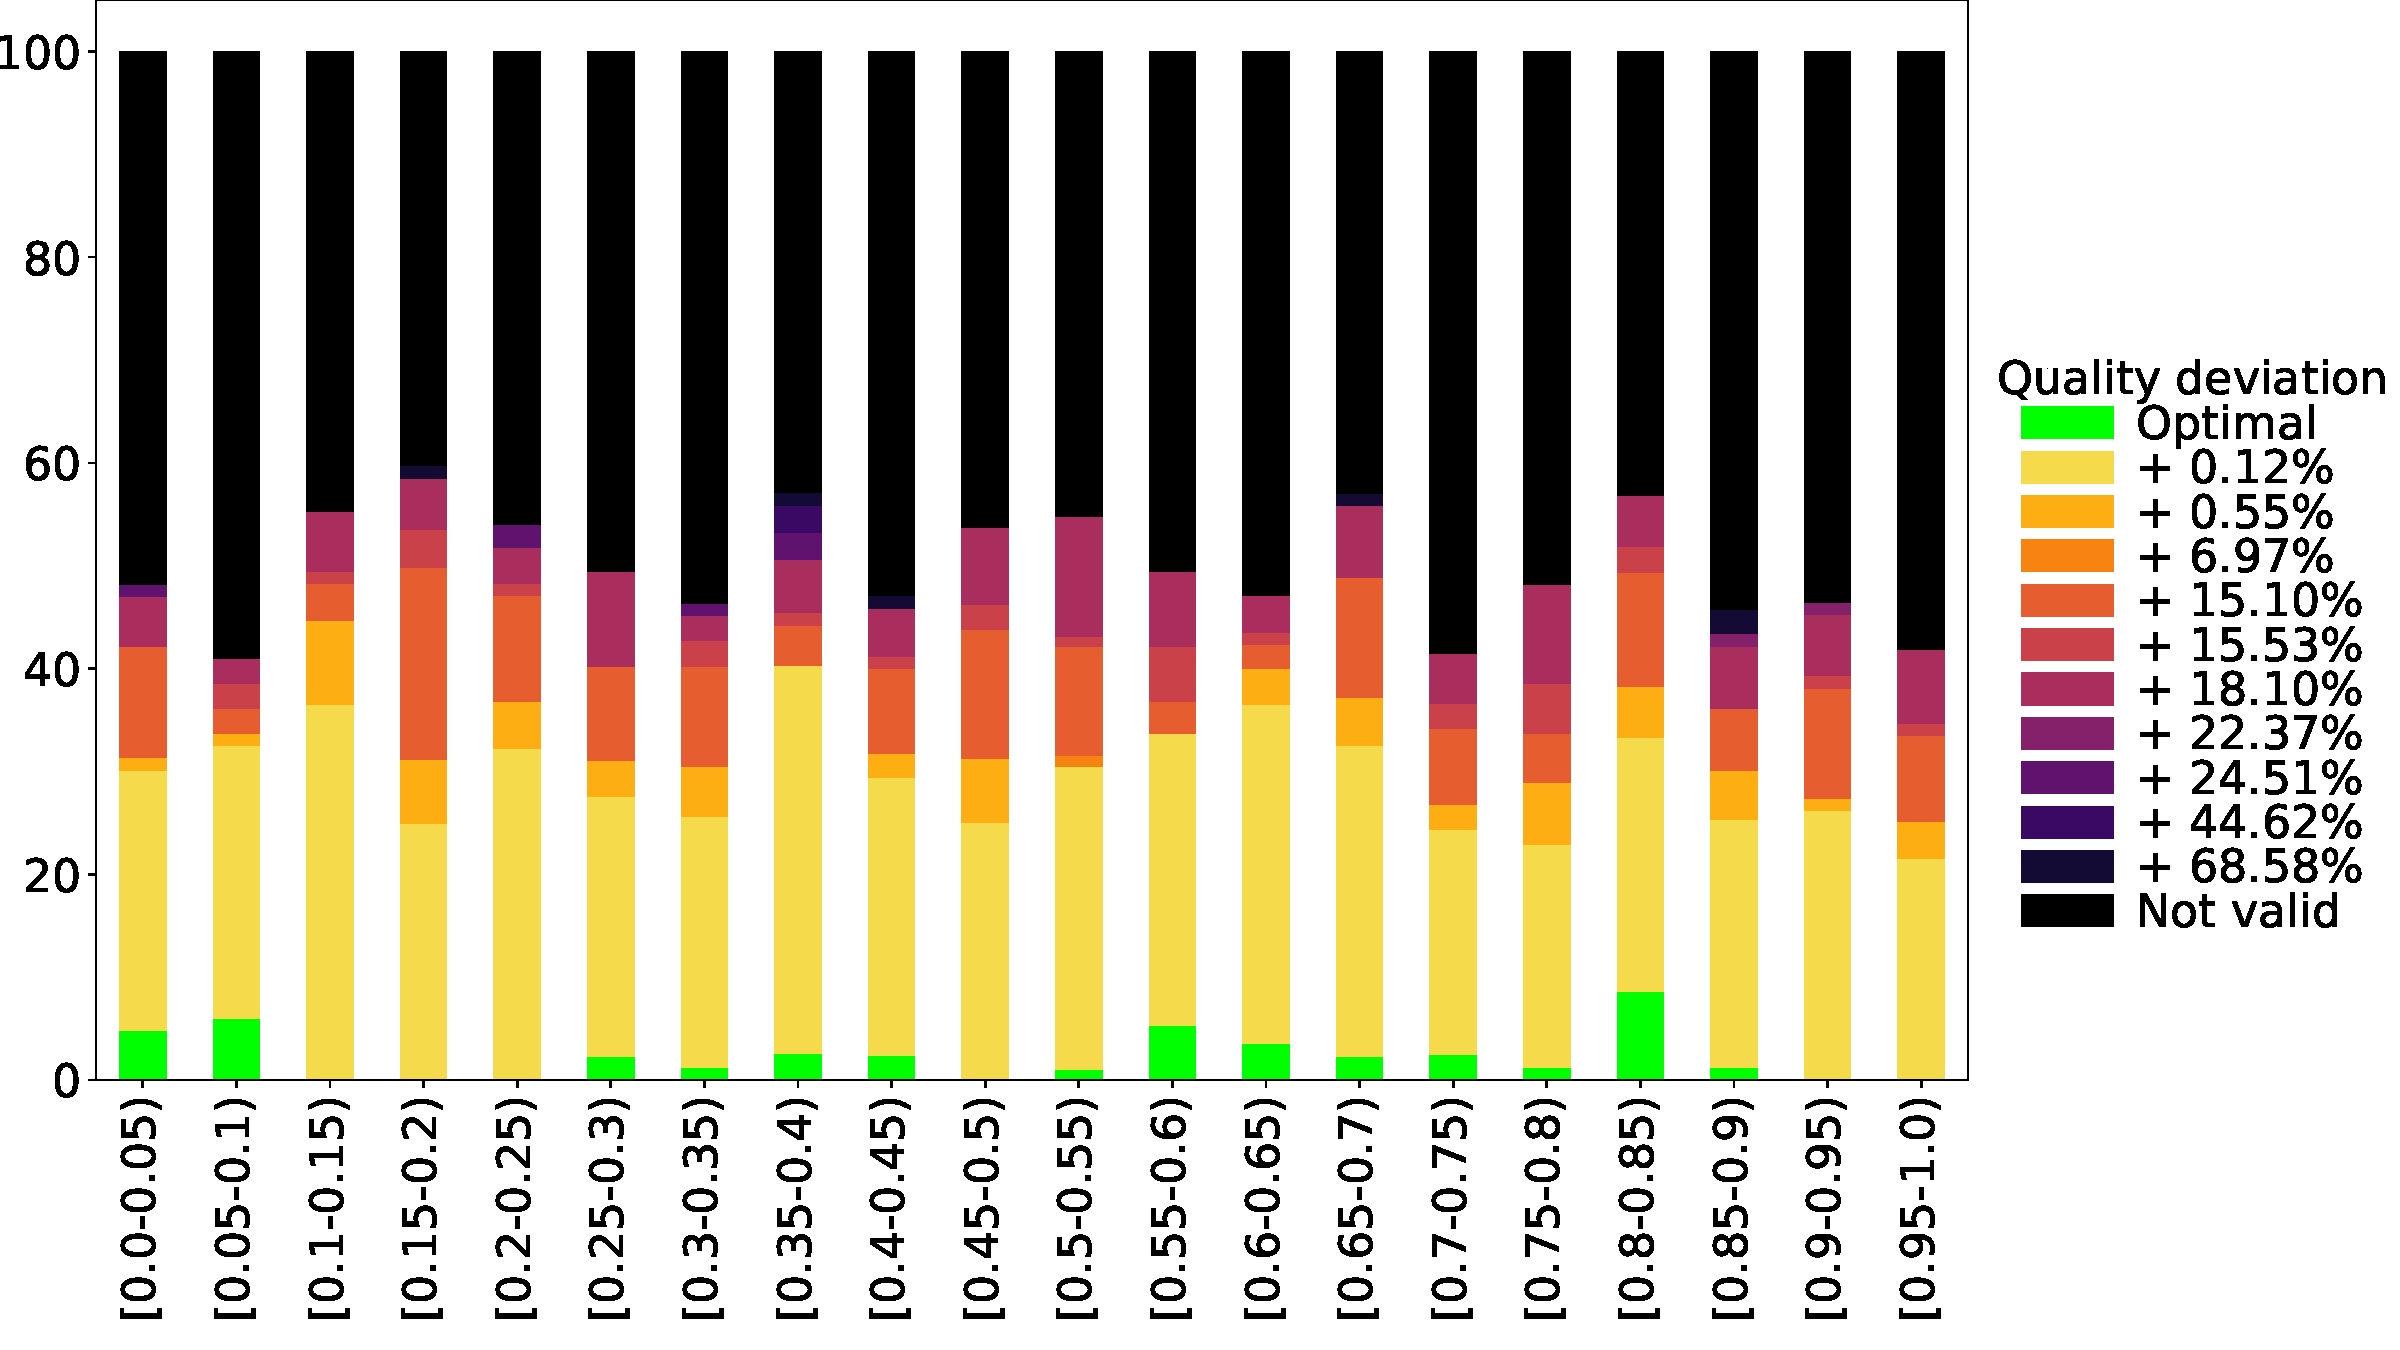
\includegraphics[width=\textwidth]{images/DistrObj/crossoverOnRandomChildProbability.pdf}
	\caption[crossoverOnRandomChildProbability parameter values distribution for smaller problem]{crossoverOnRandomChildProbability parameter values distribution for smaller problem}
	\label{fig:crossoverOnRandomChildProbability_Obj}
\end{figure}
\begin{figure}
	\centering
	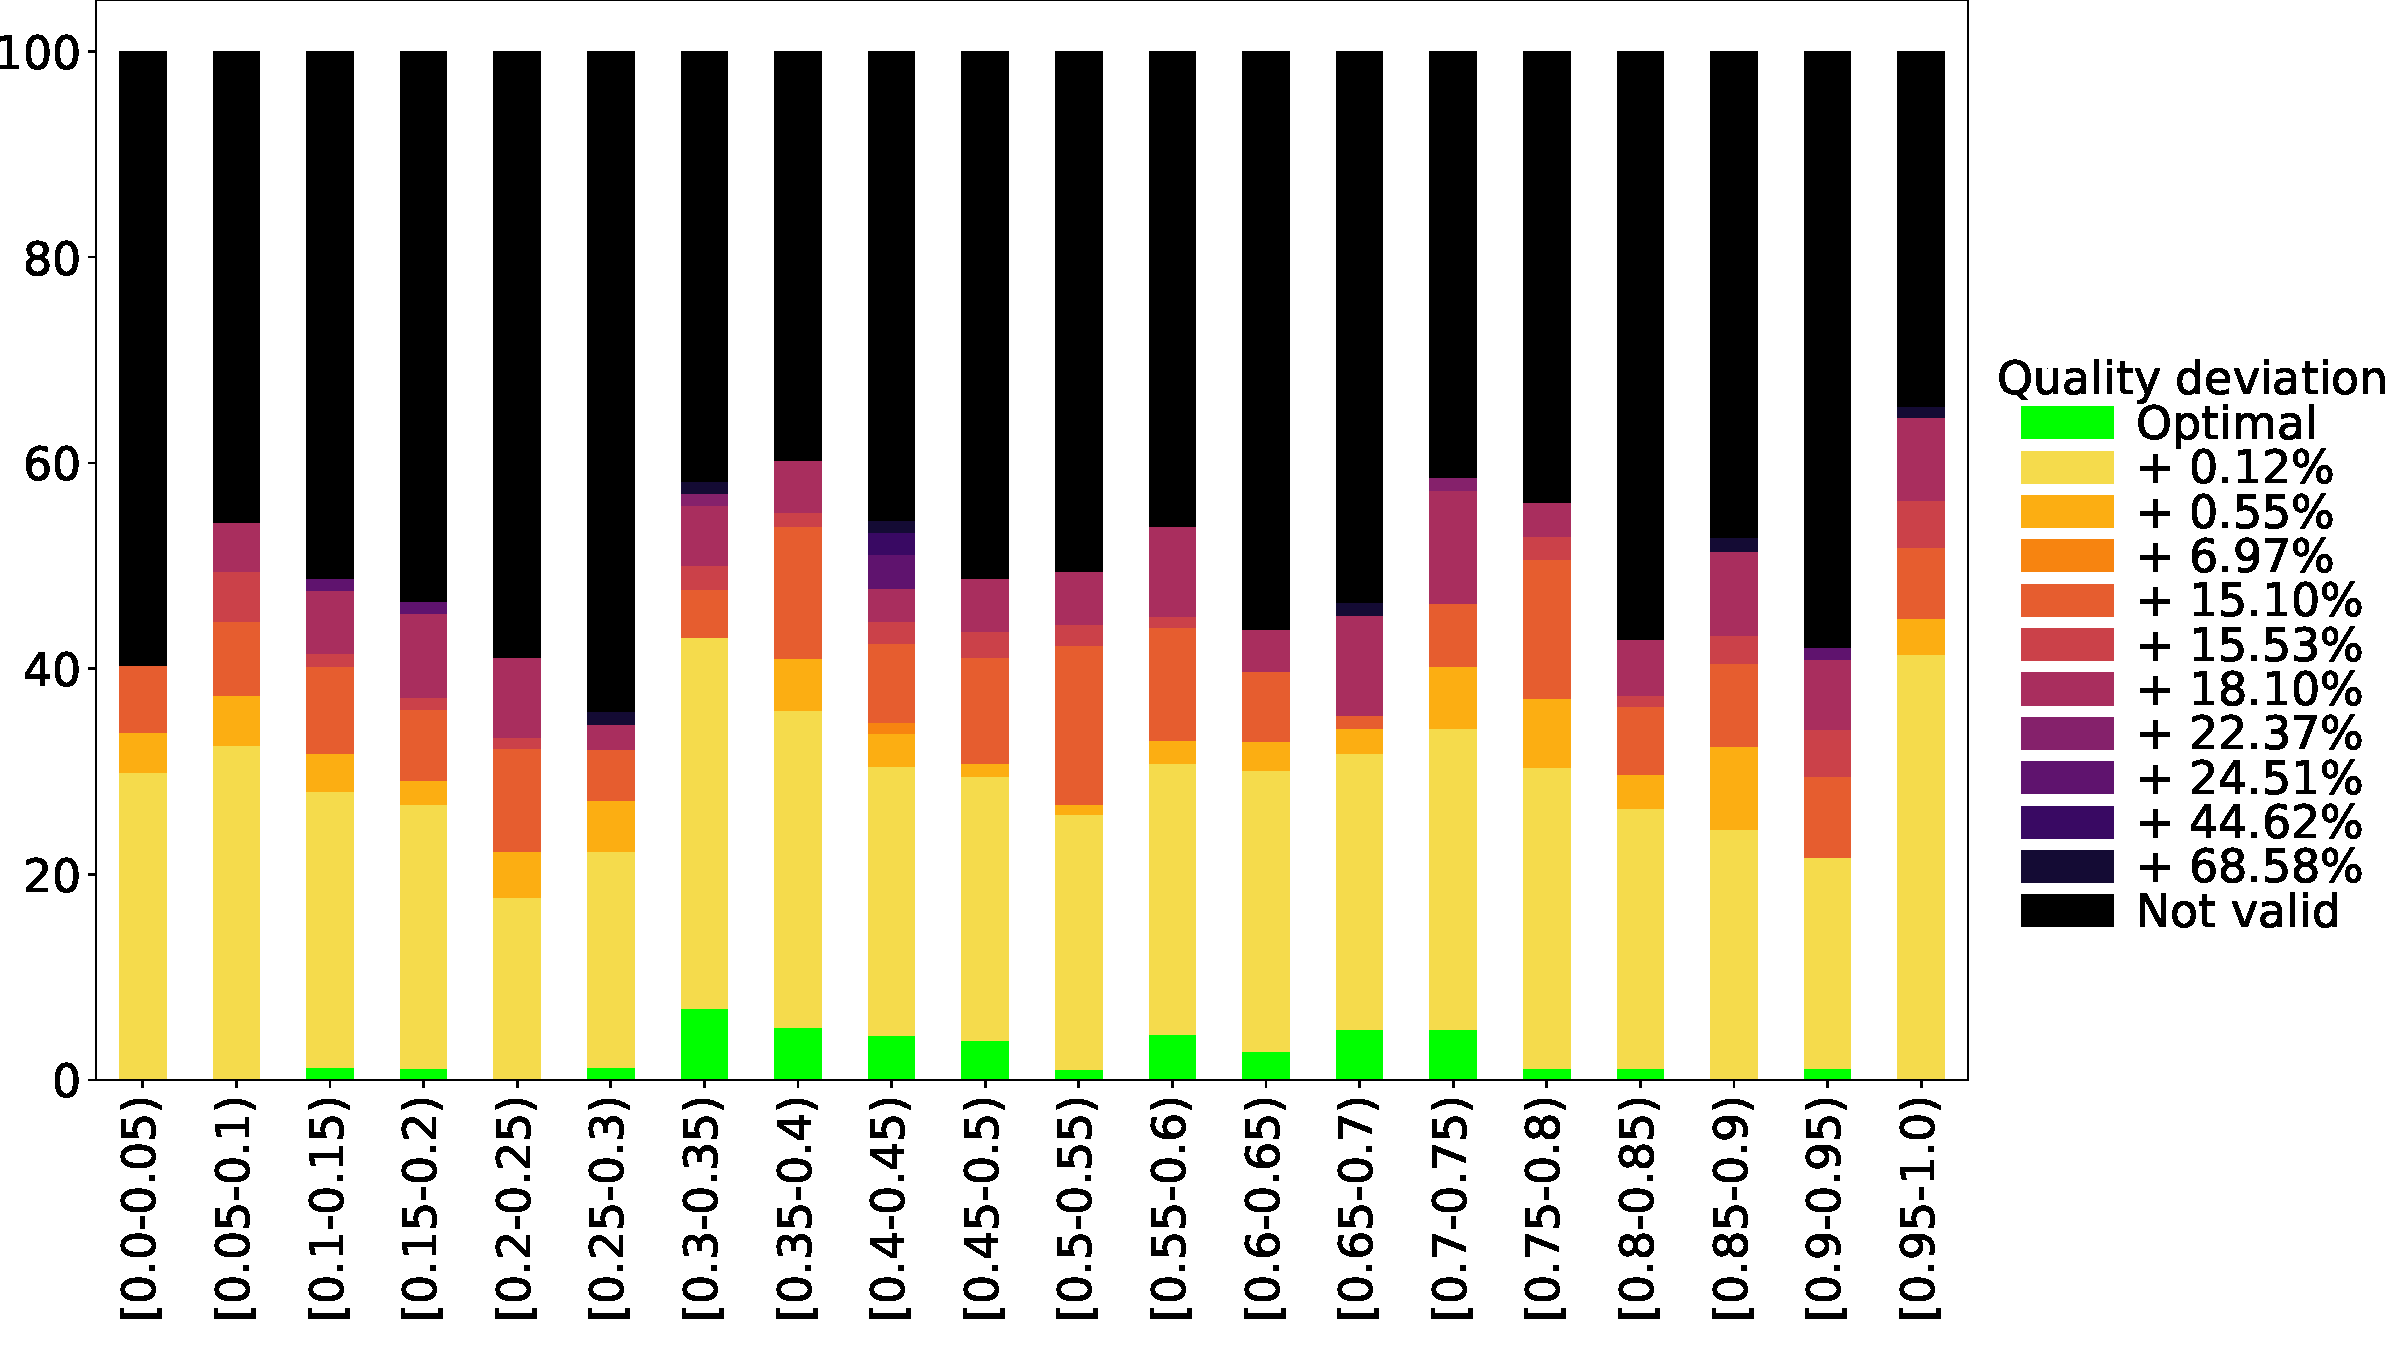
\includegraphics[width=\textwidth]{images/DistrObj/crossoverOnRandomLevelProbability.pdf}
	\caption[crossoverOnRandomLevelProbability parameter values distribution for smaller problem]{crossoverOnRandomLevelProbability parameter values distribution for smaller problem}
	\label{fig:crossoverOnRandomLevelProbability_Obj}
\end{figure}
\begin{figure}
	\centering
	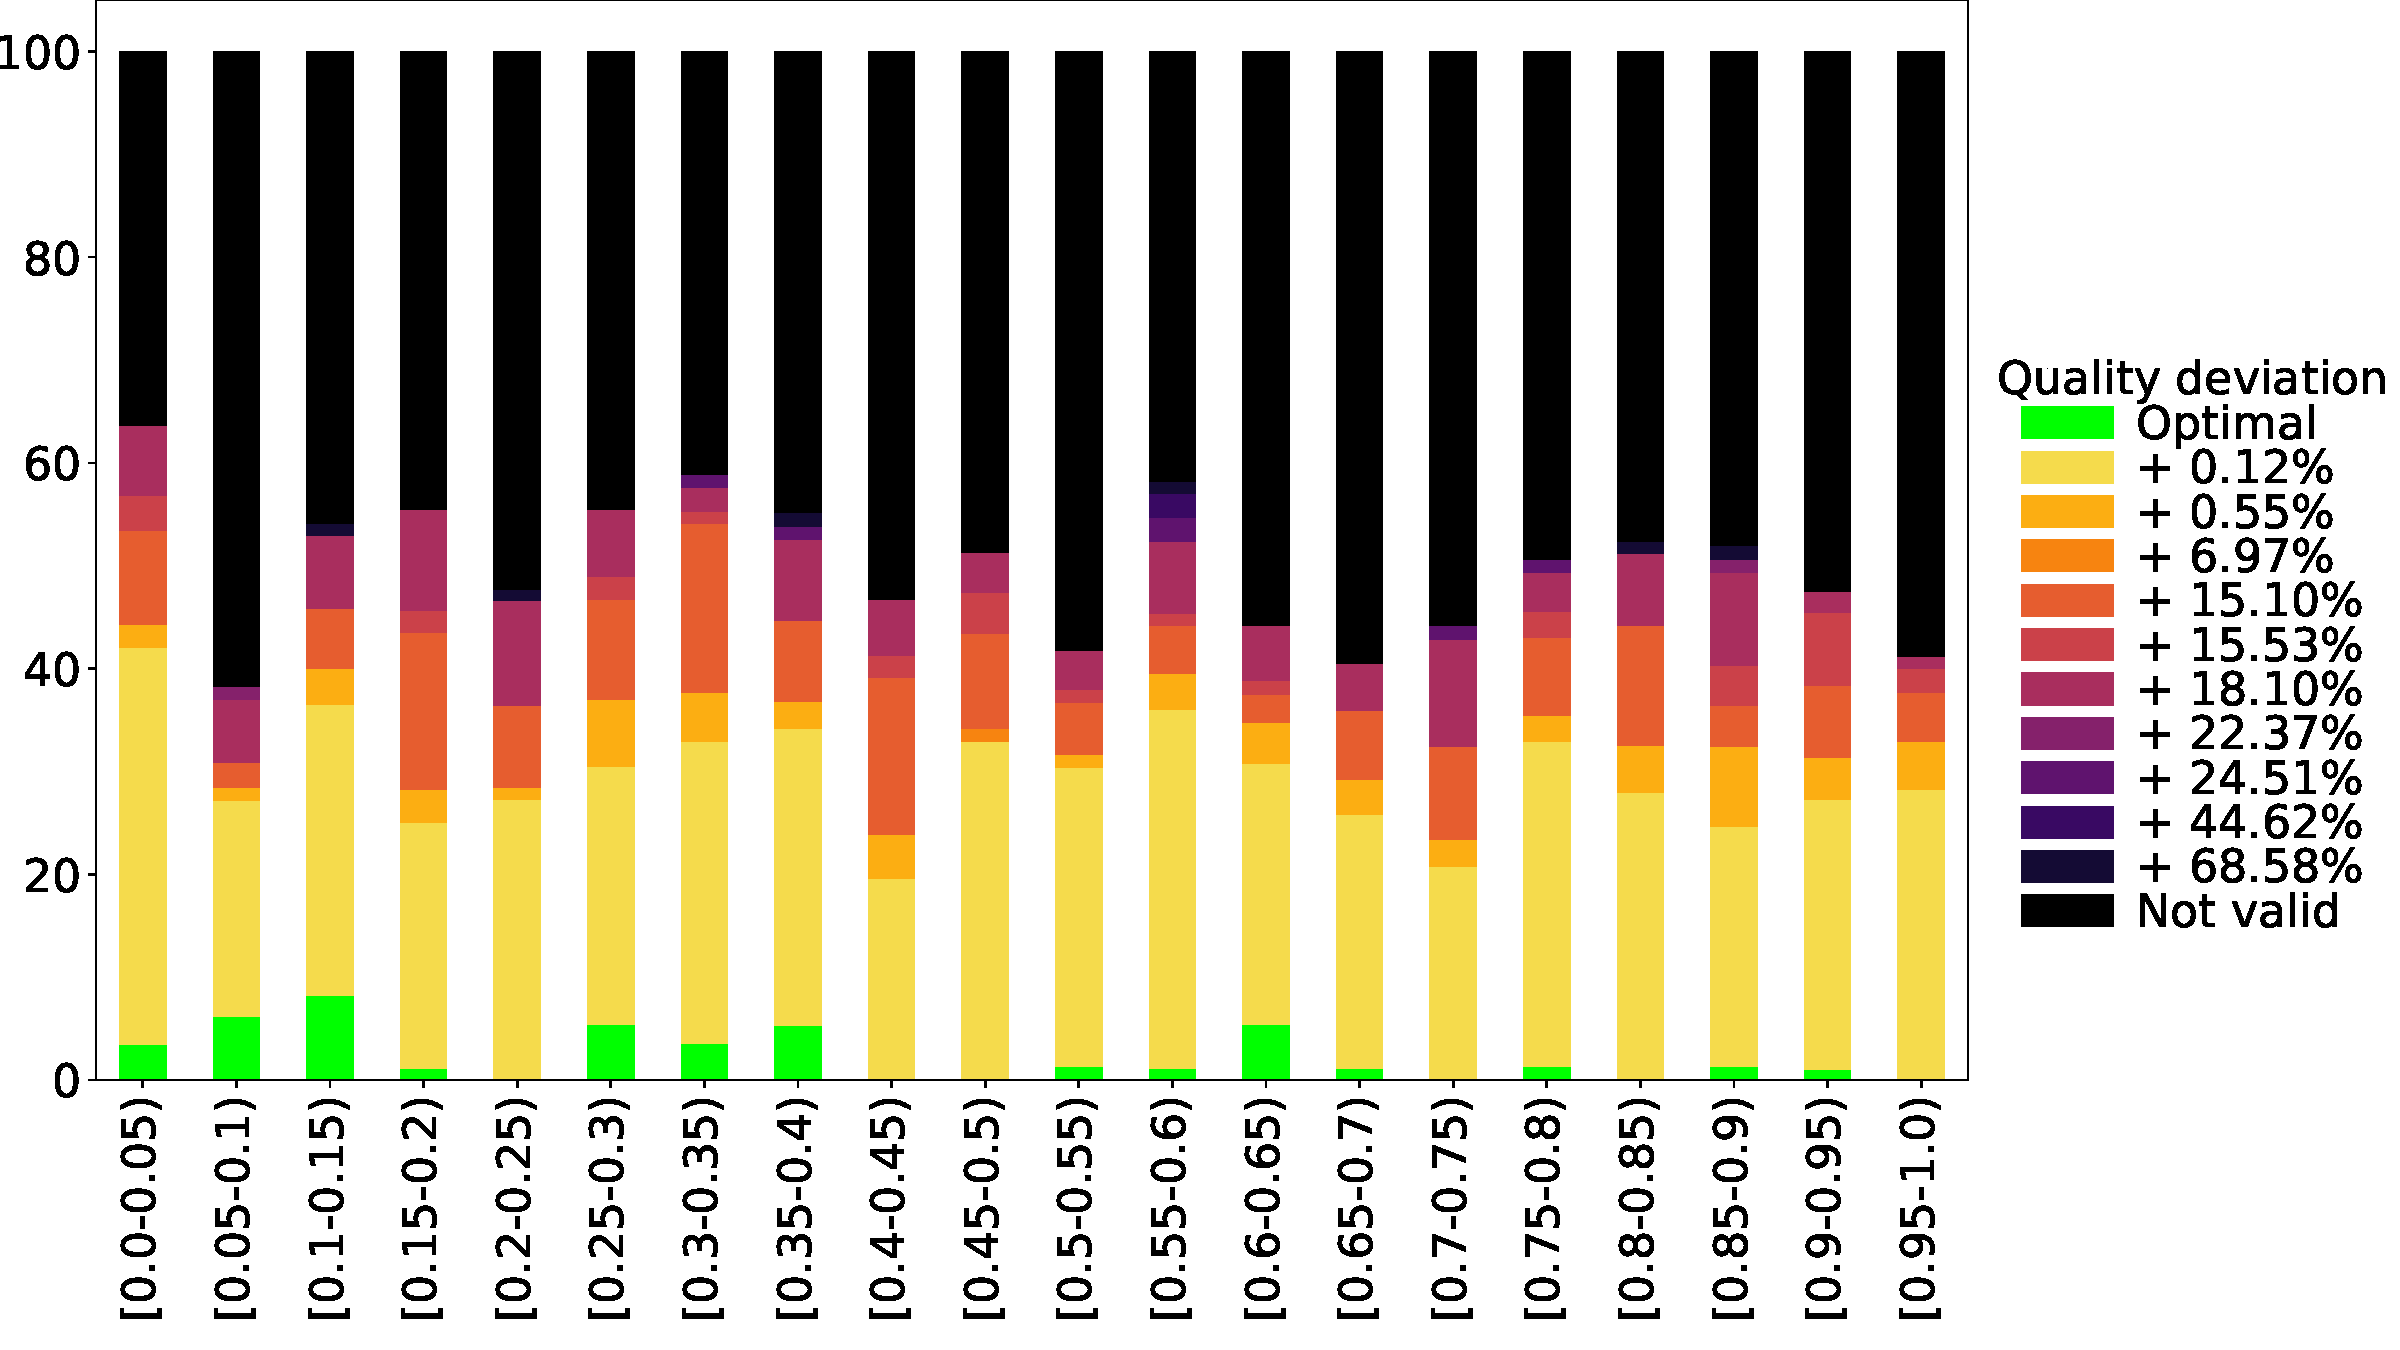
\includegraphics[width=\textwidth]{images/DistrObj/crossoverOnRandomRequestProbability.pdf}
	\caption[crossoverOnRandomRequestProbability parameter values distribution for smaller problem]{crossoverOnRandomRequestProbability parameter values distribution for smaller problem}       
	\label{fig:crossoverOnRandomRequestProbability_Obj}
\end{figure}
\begin{figure}
	\centering
	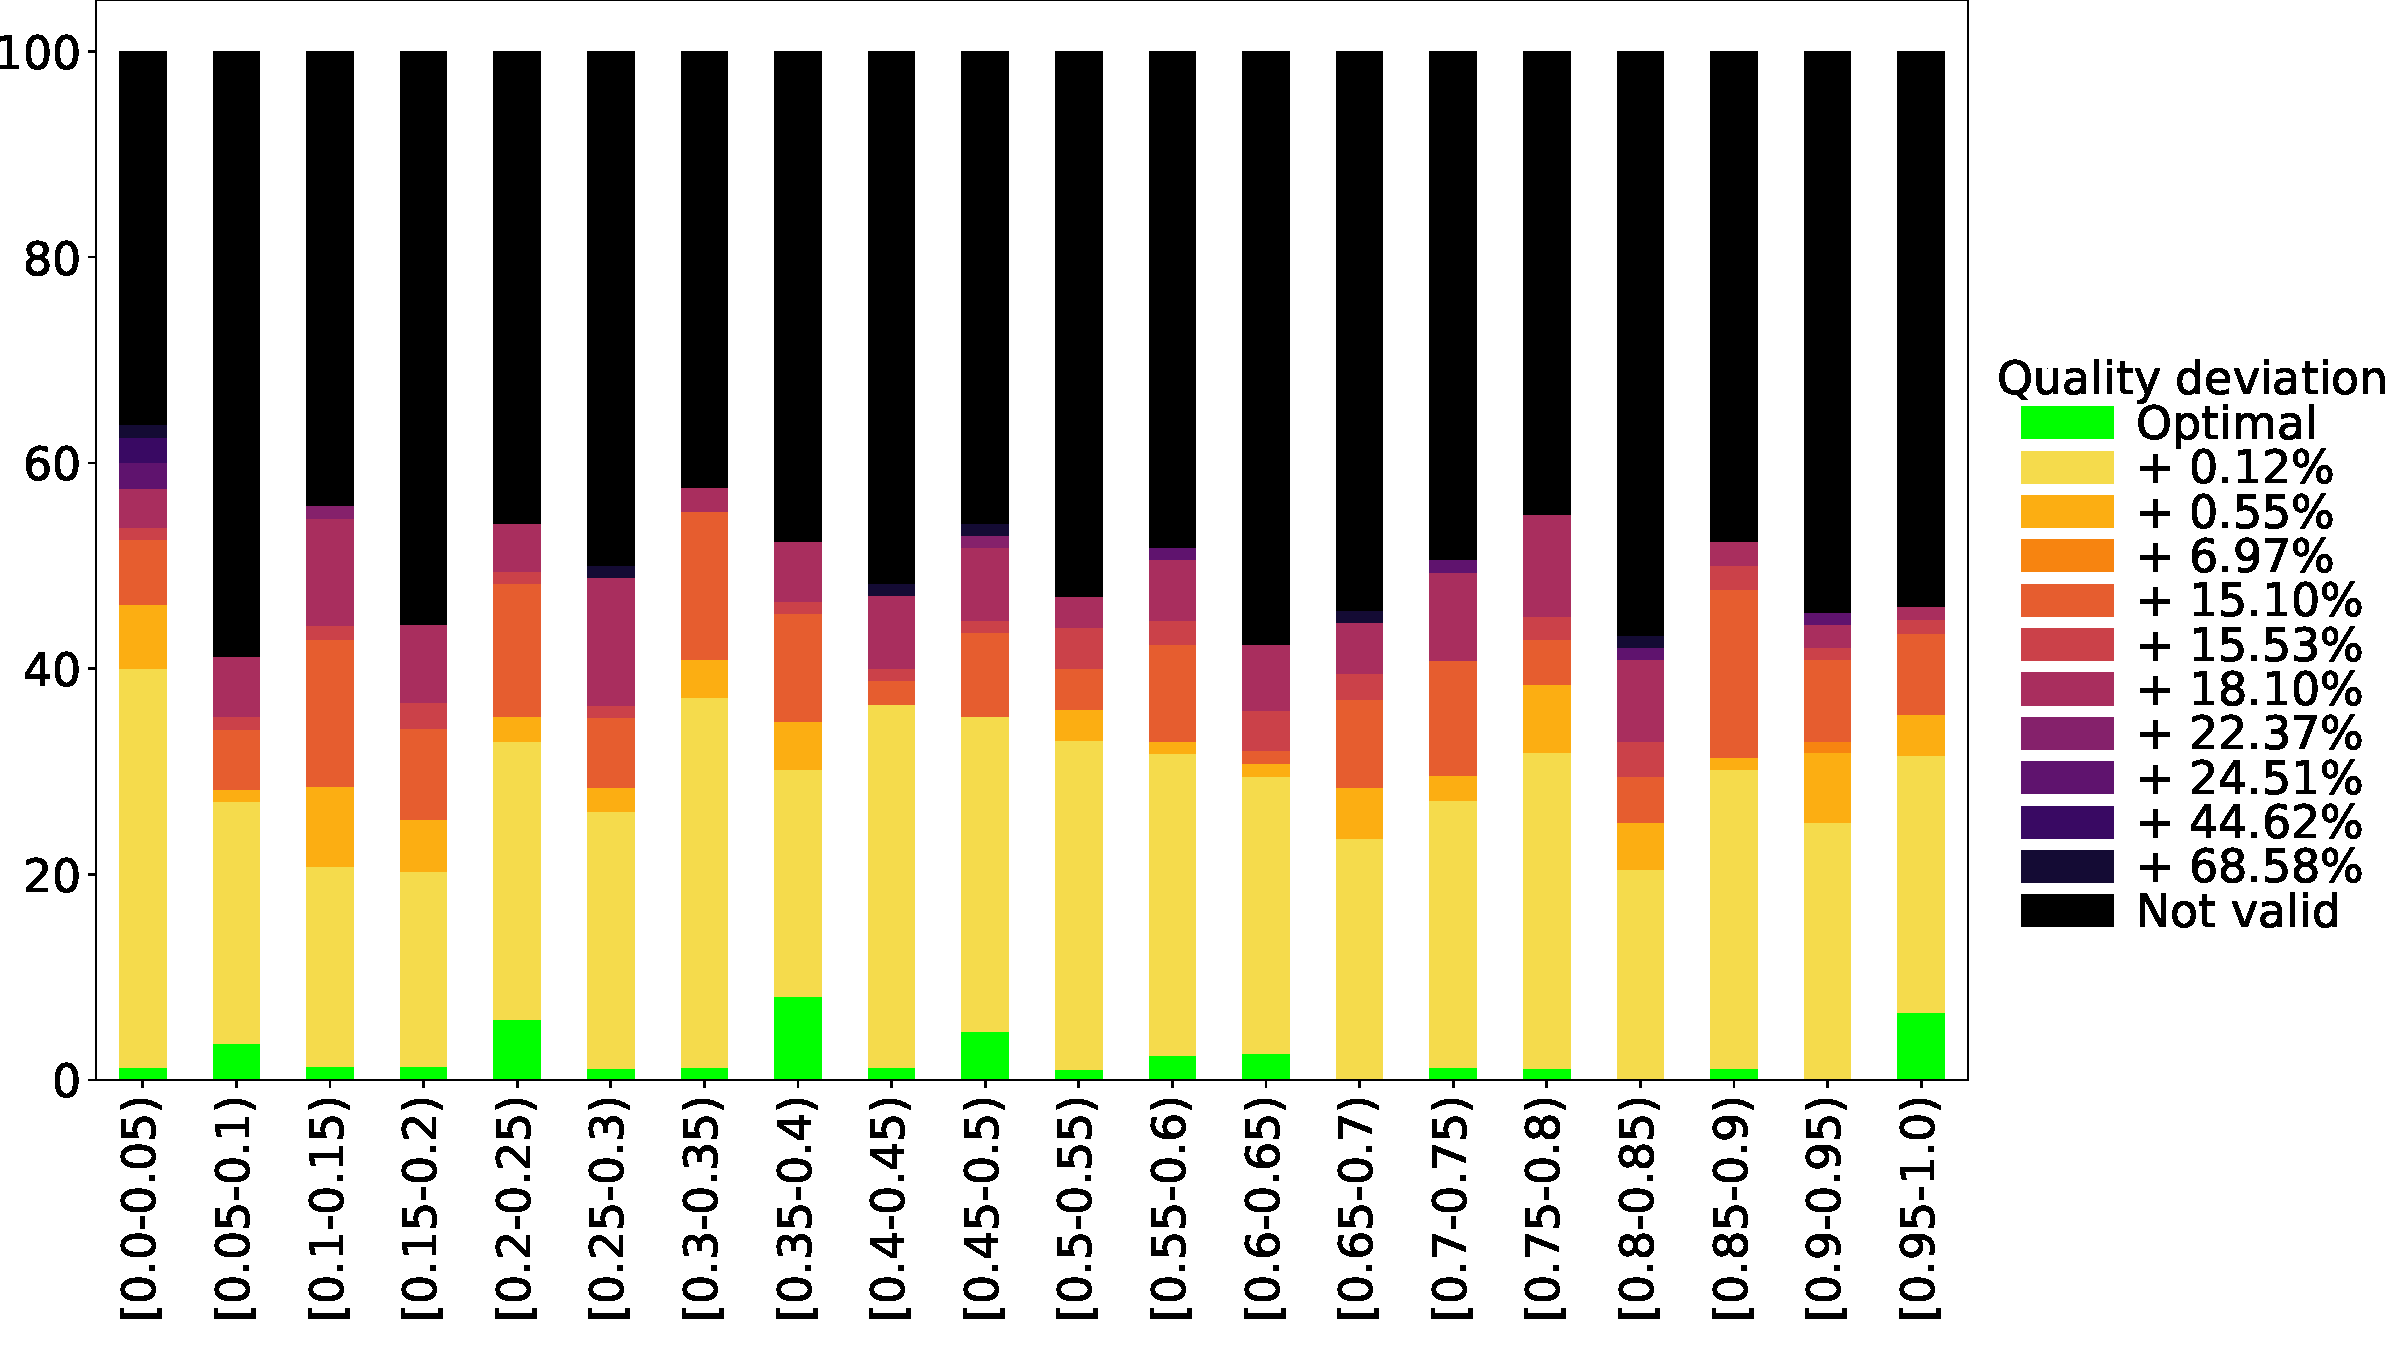
\includegraphics[width=\textwidth]{images/DistrObj/mutationOnRandomChildProbability.pdf}
	\caption[mutationOnRandomChildProbability parameter values distribution for smaller problem]{mutationOnRandomChildProbability parameter values distribution for smaller problem}
	\label{fig:mutationOnRandomChildProbability_Obj}
\end{figure}
\begin{figure}
	\centering
	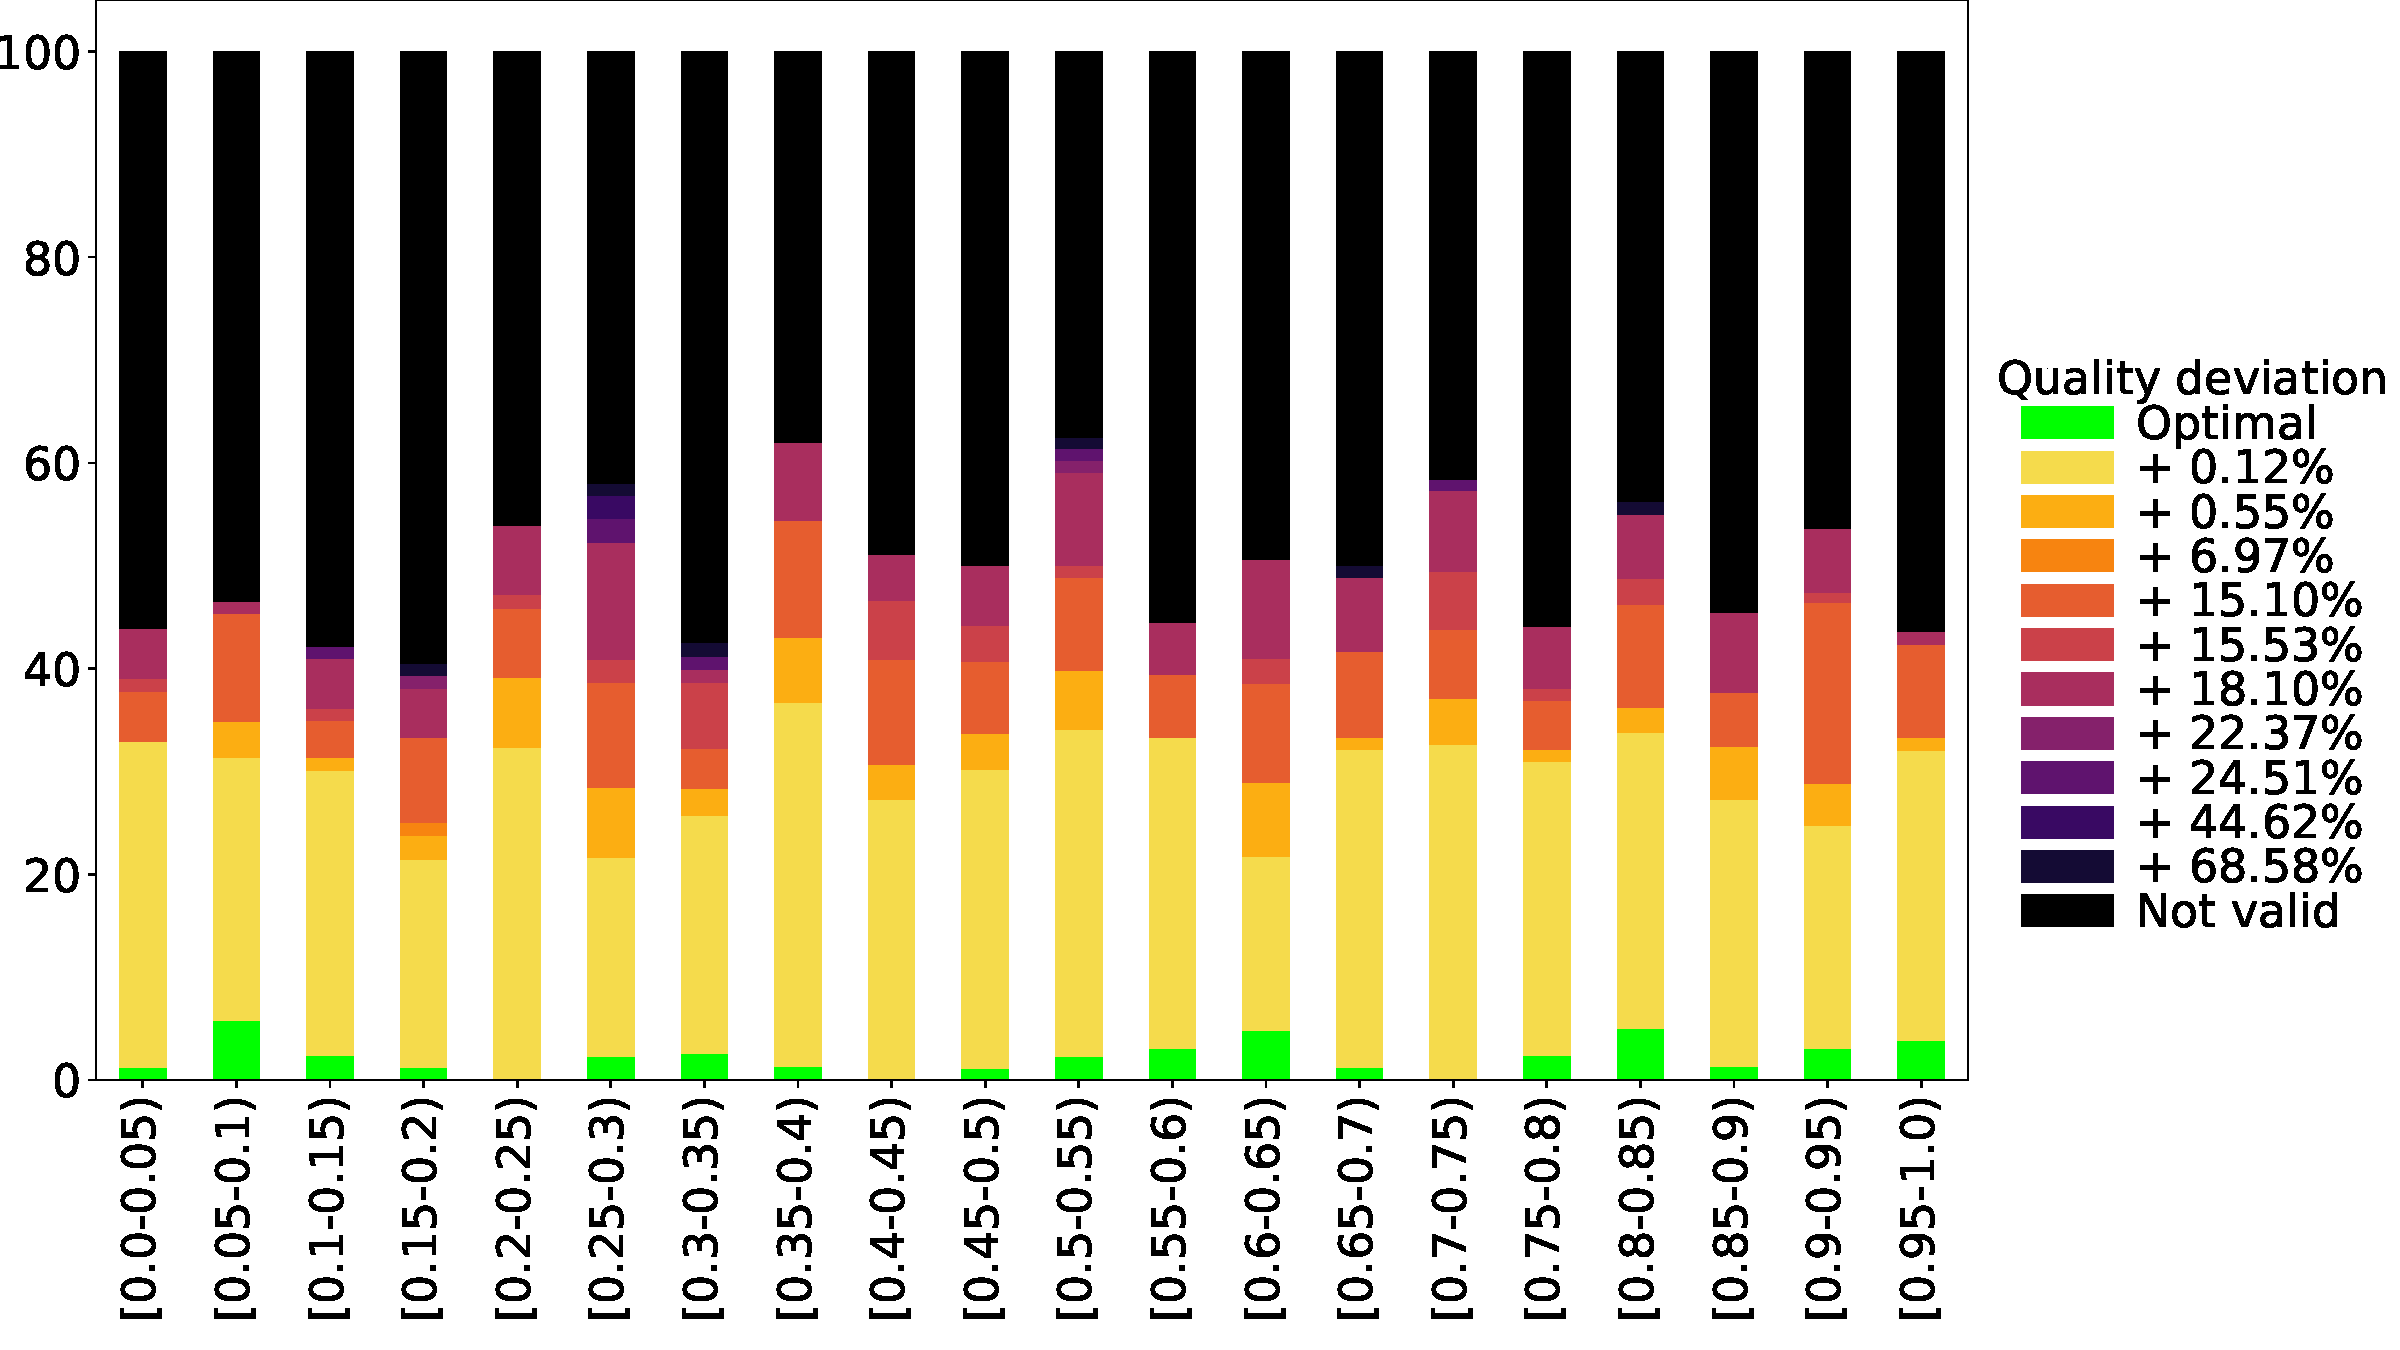
\includegraphics[width=\textwidth]{images/DistrObj/mutationOnRandomLevelProbability.pdf}
	\caption[mutationOnRandomLevelProbability parameter values distribution for smaller problem]{mutationOnRandomLevelProbability parameter values distribution for smaller problem}
	\label{fig:mutationOnRandomLevelProbability_Obj}
\end{figure}
\begin{figure}
	\centering
	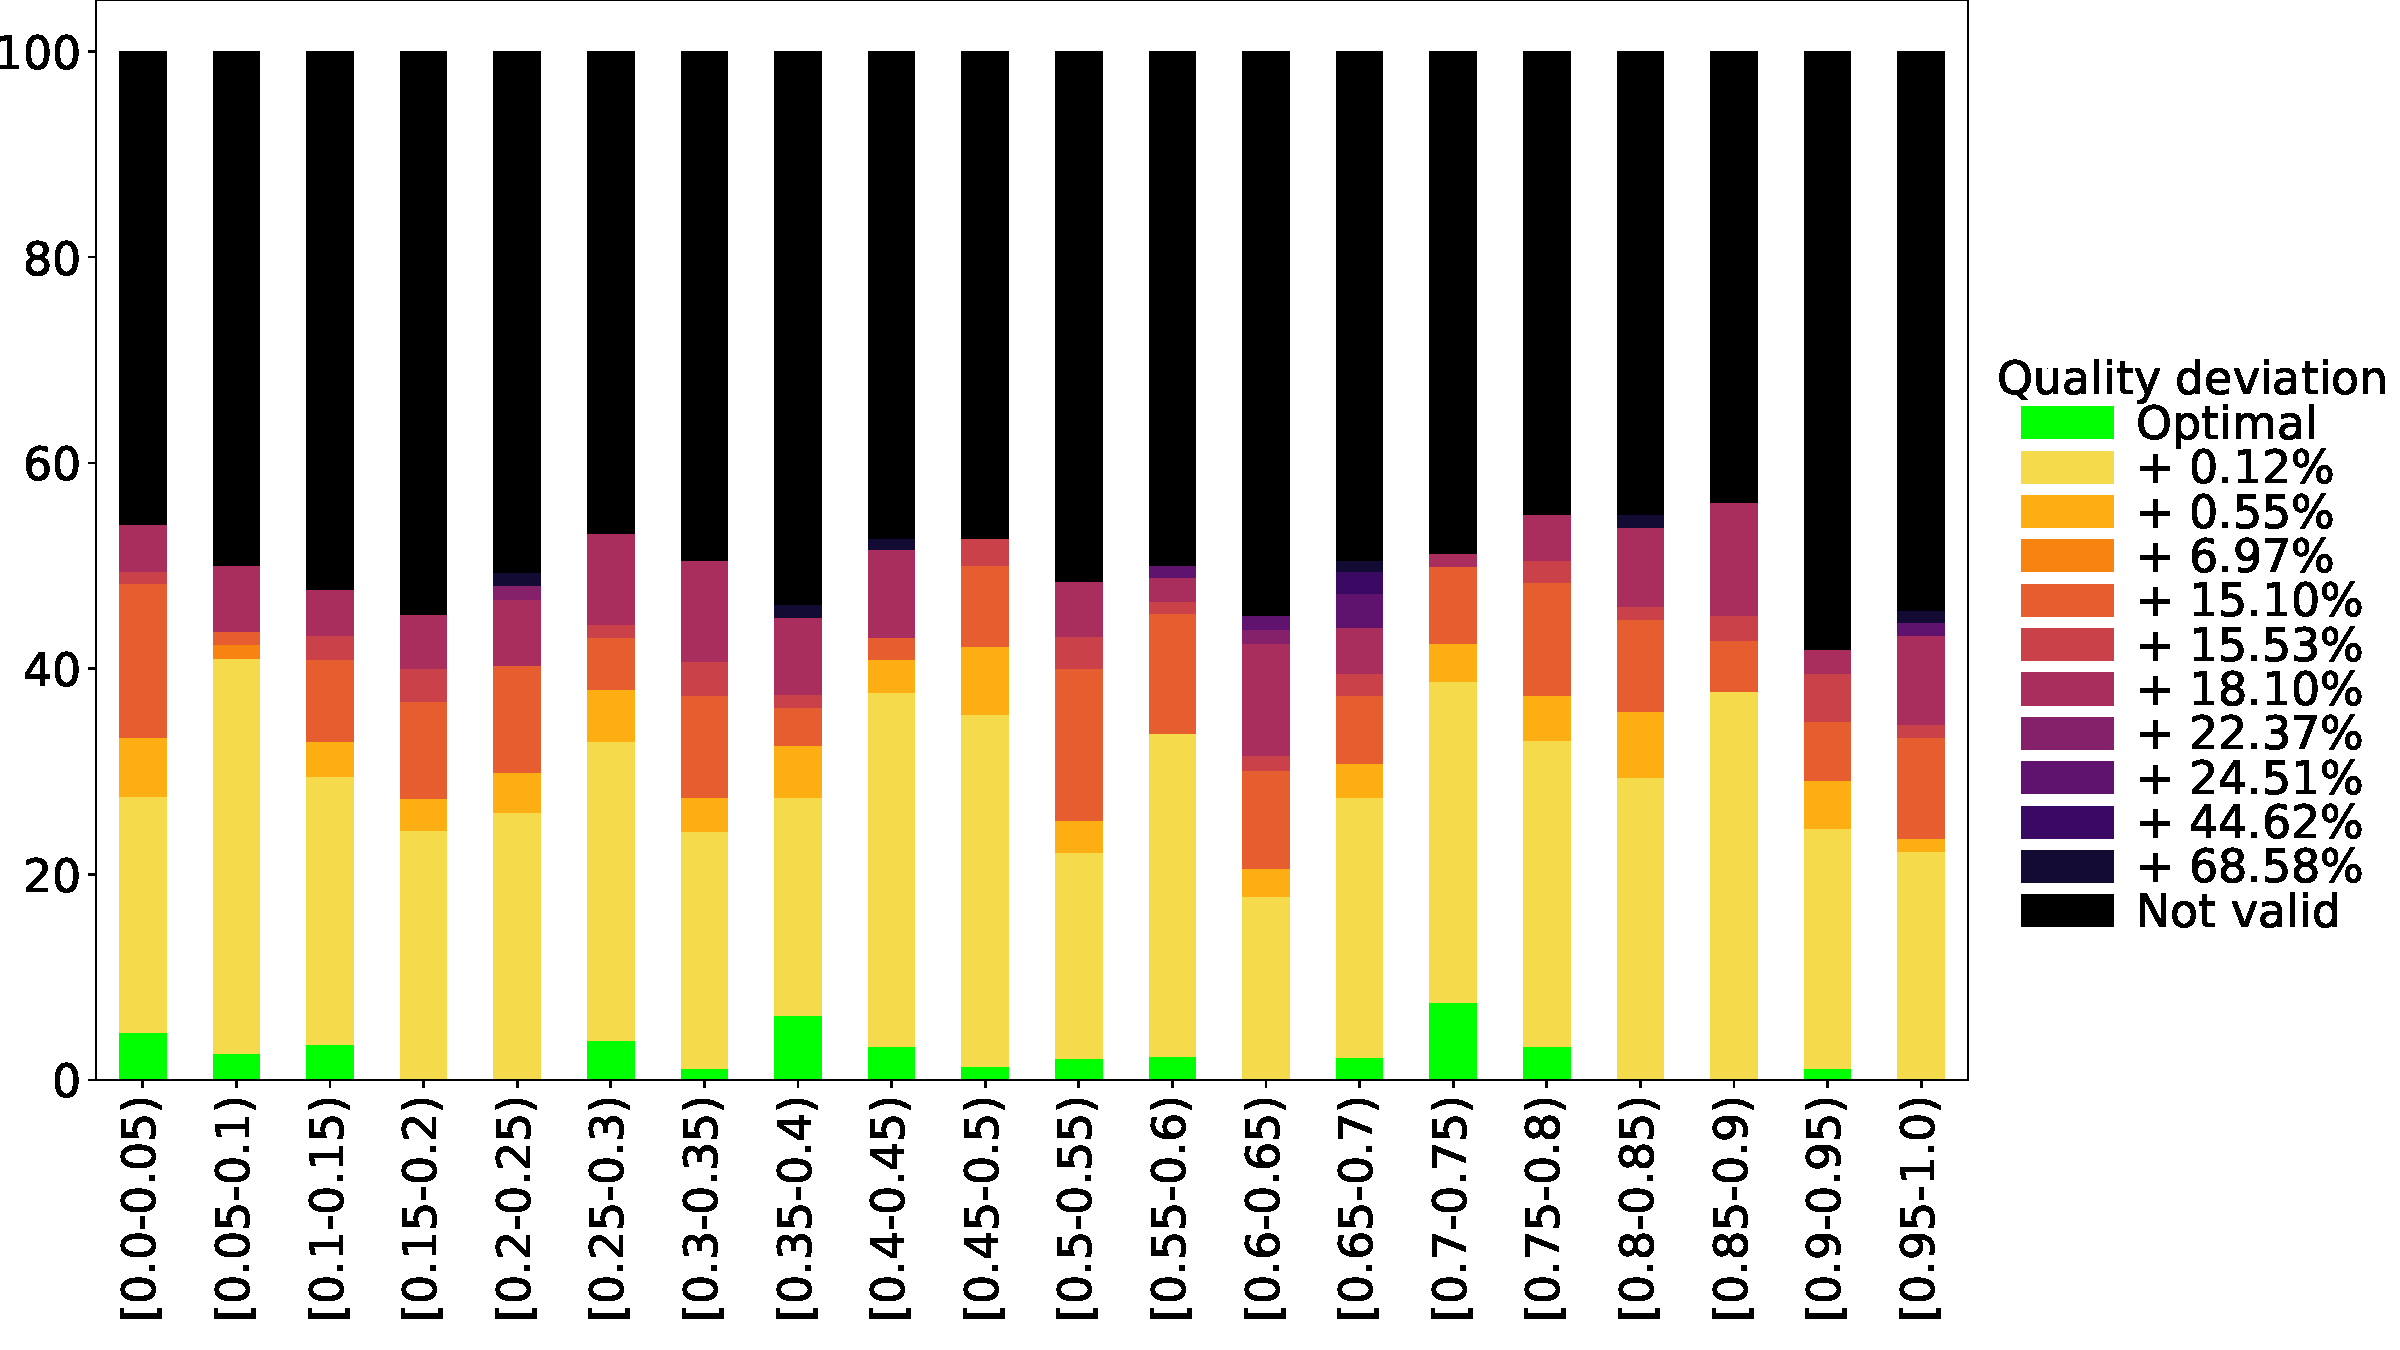
\includegraphics[width=\textwidth]{images/DistrObj/evaluatorValidityWeight.pdf}
	\caption[evaluatorValidityWeight parameter values distribution for smaller problem]{evaluatorValidityWeight parameter values distribution for smaller problem}
	\label{fig:evaluatorValidityWeight_Obj}
\end{figure}
\begin{figure}
	\centering
	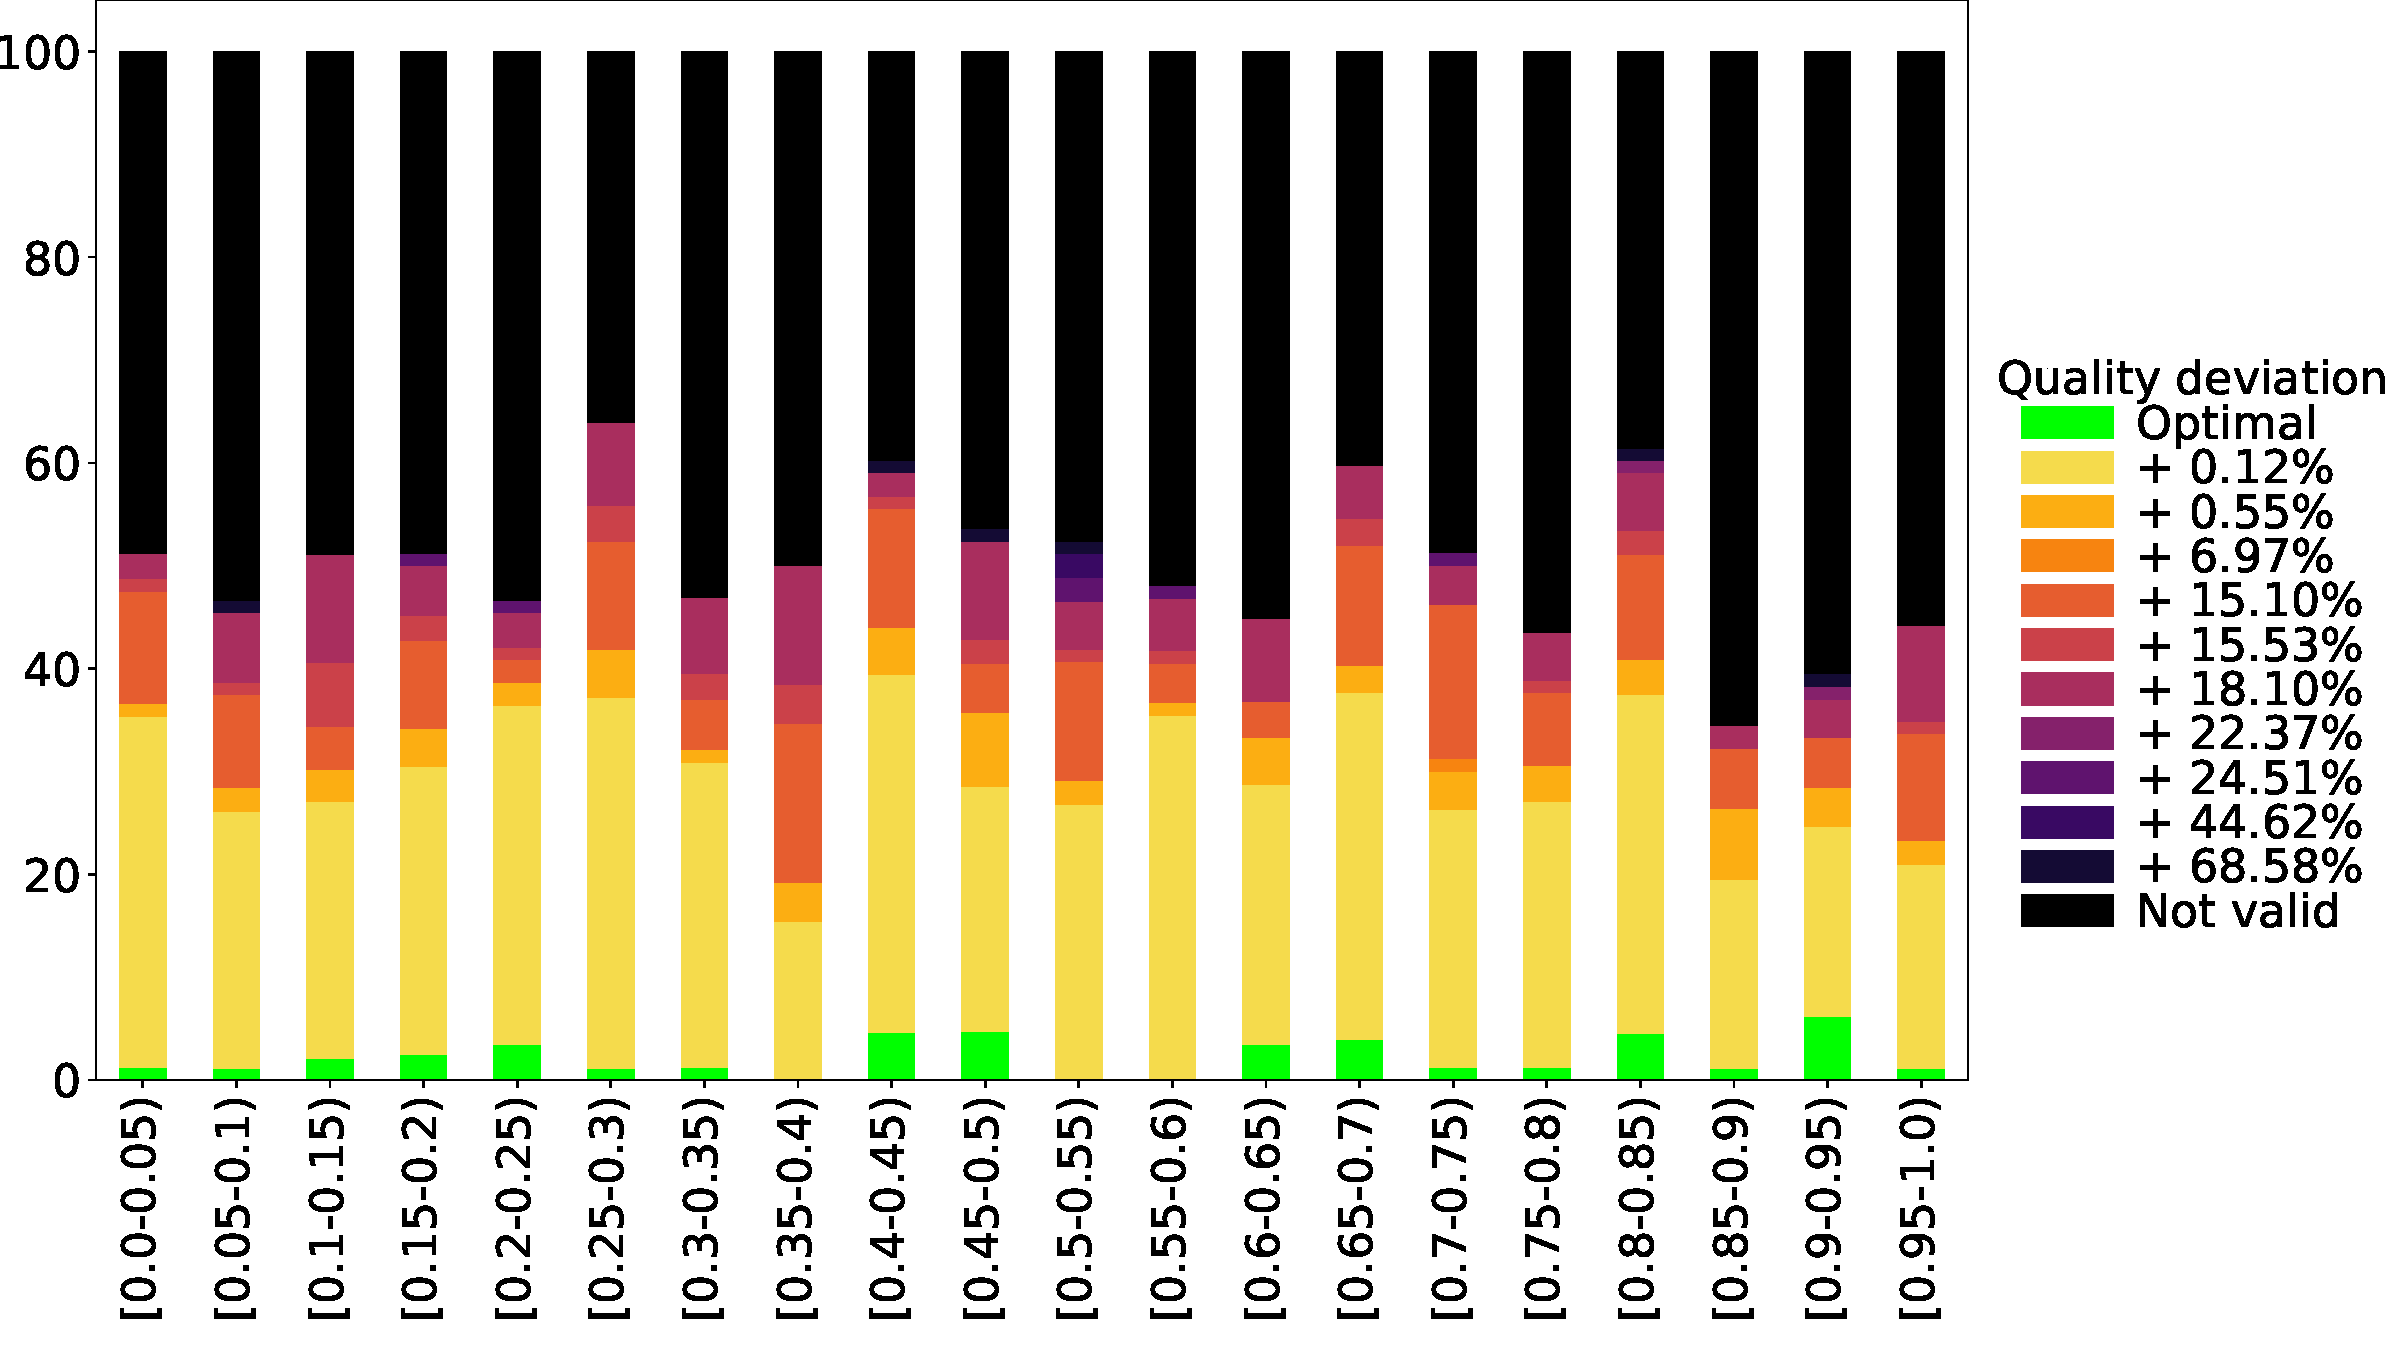
\includegraphics[width=\textwidth]{images/DistrObj/evaluatorSoftwareValidityWeight.pdf}
	\caption[evaluatorSoftwareValidityWeight parameter values distribution for smaller problem]{evaluatorSoftwareValidityWeight parameter values distribution for smaller problem}
	\label{fig:evaluatorSoftwareValidityWeight_Obj}
\end{figure}
\begin{figure}
	\centering
	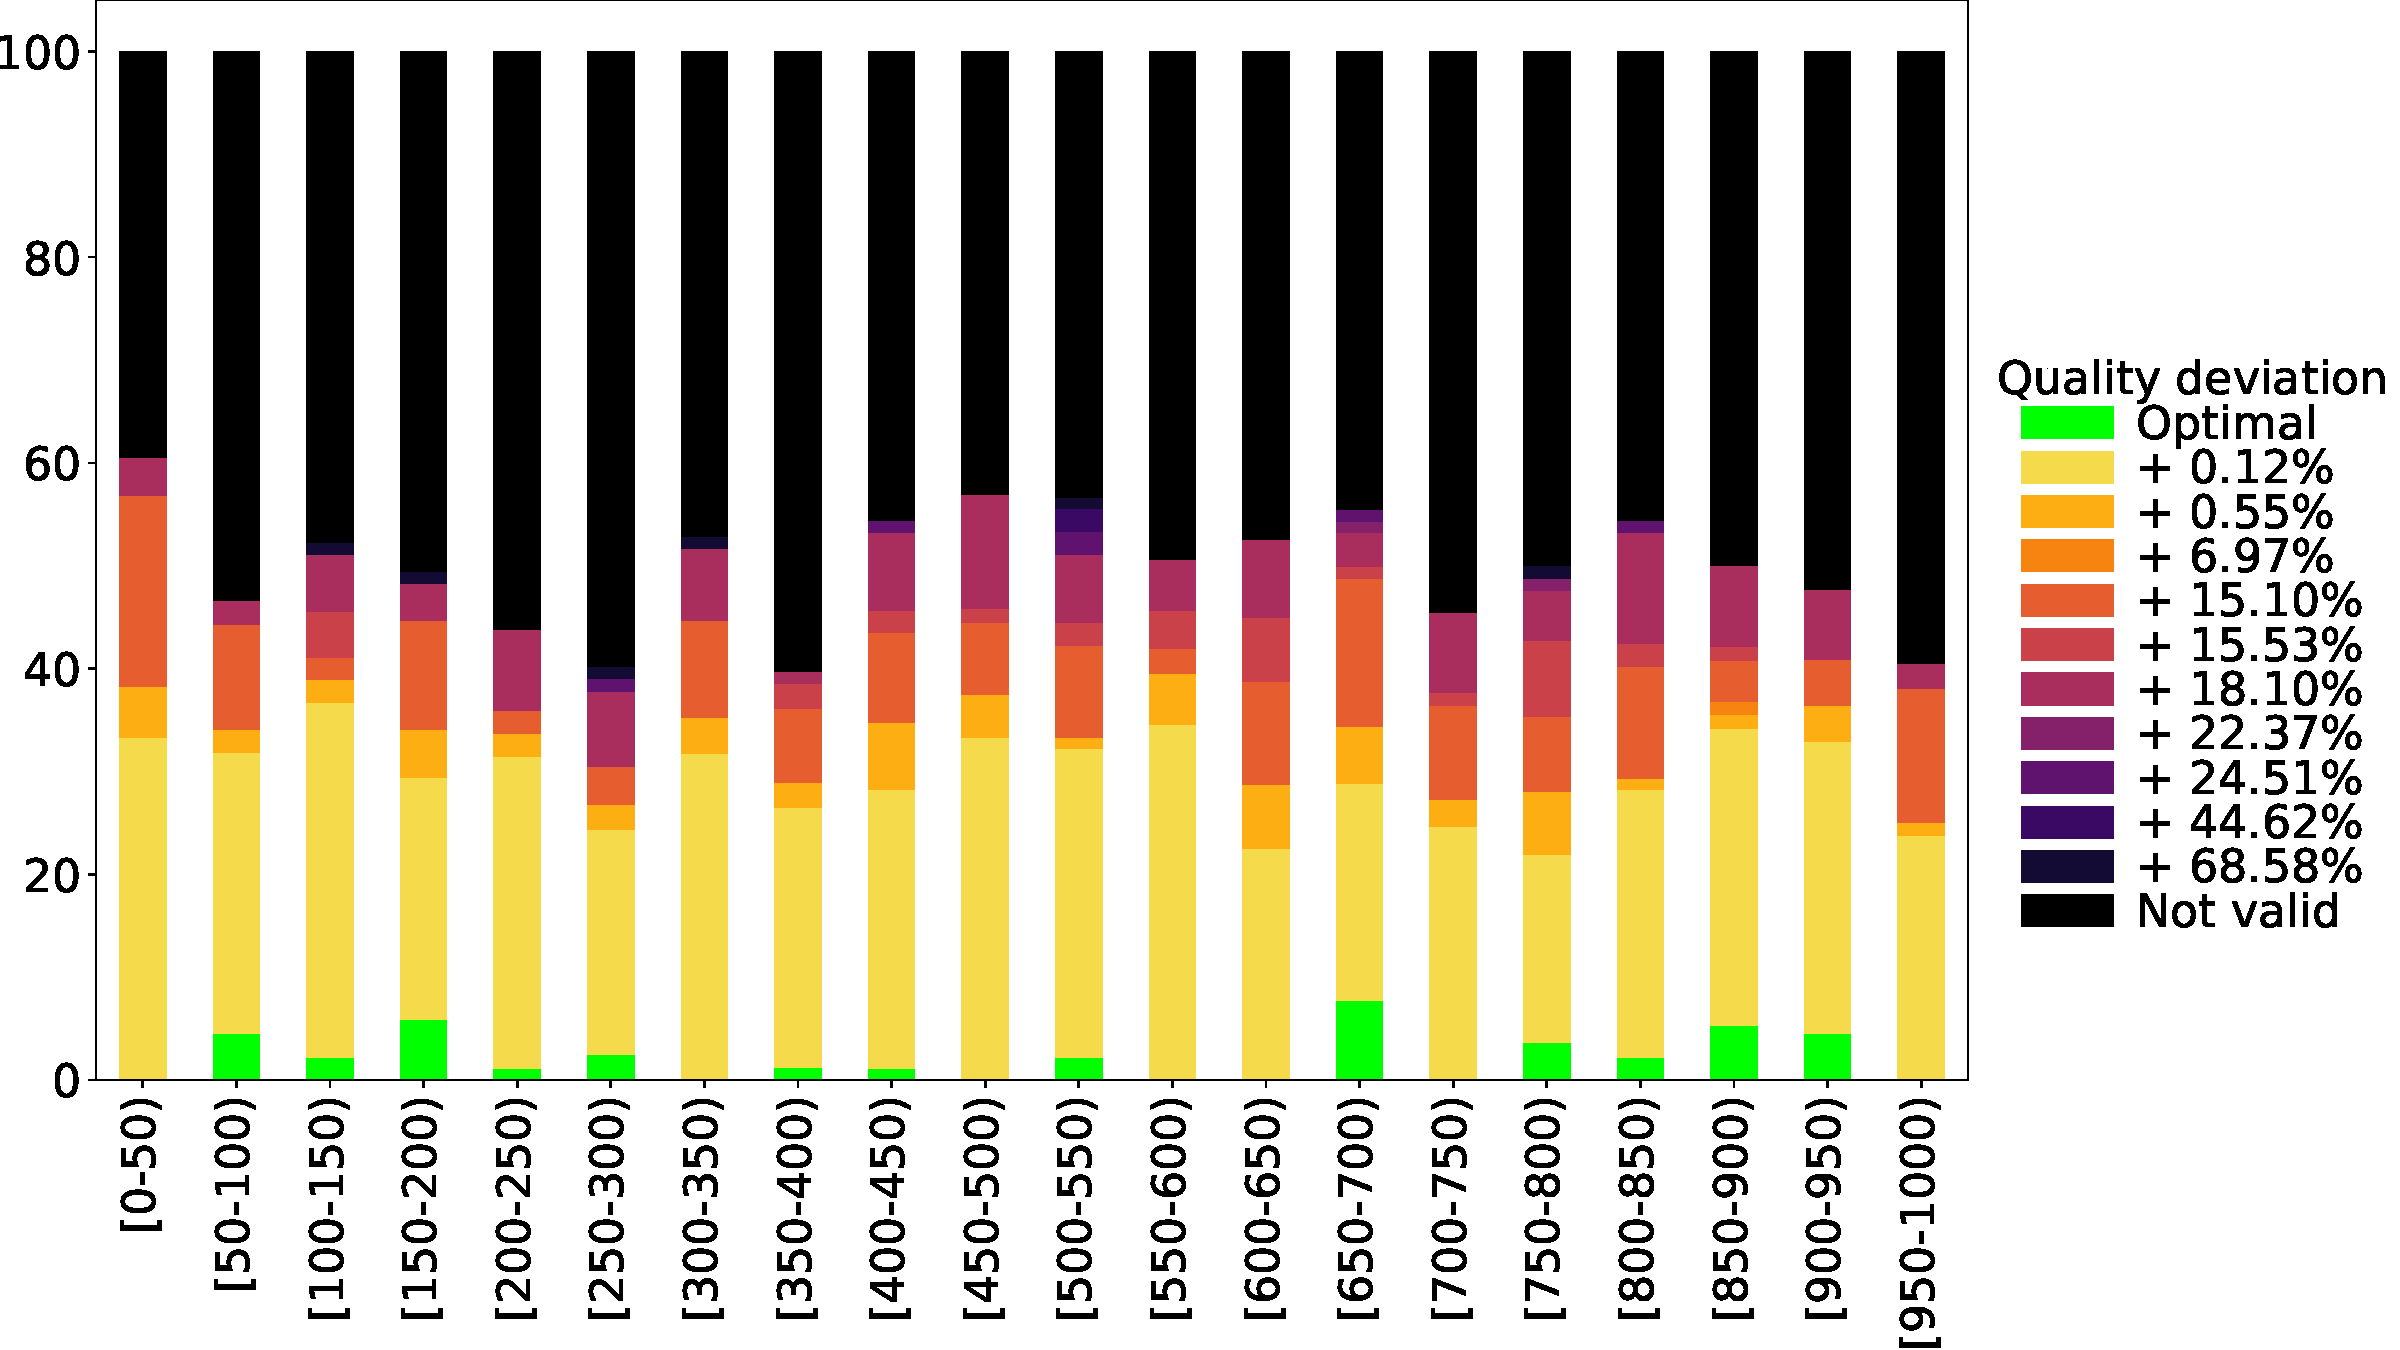
\includegraphics[width=\textwidth]{images/DistrObj/randomSoftwareAssignmentAttempts.pdf}
	\caption[randomSoftwareAssignmentAttempts parameter values distribution for smaller problem]{randomSoftwareAssignmentAttempts parameter values distribution for smaller problem}
	\label{fig:randomSoftwareAssignmentAttempts_Obj}
\end{figure}
\begin{figure}
	\centering
	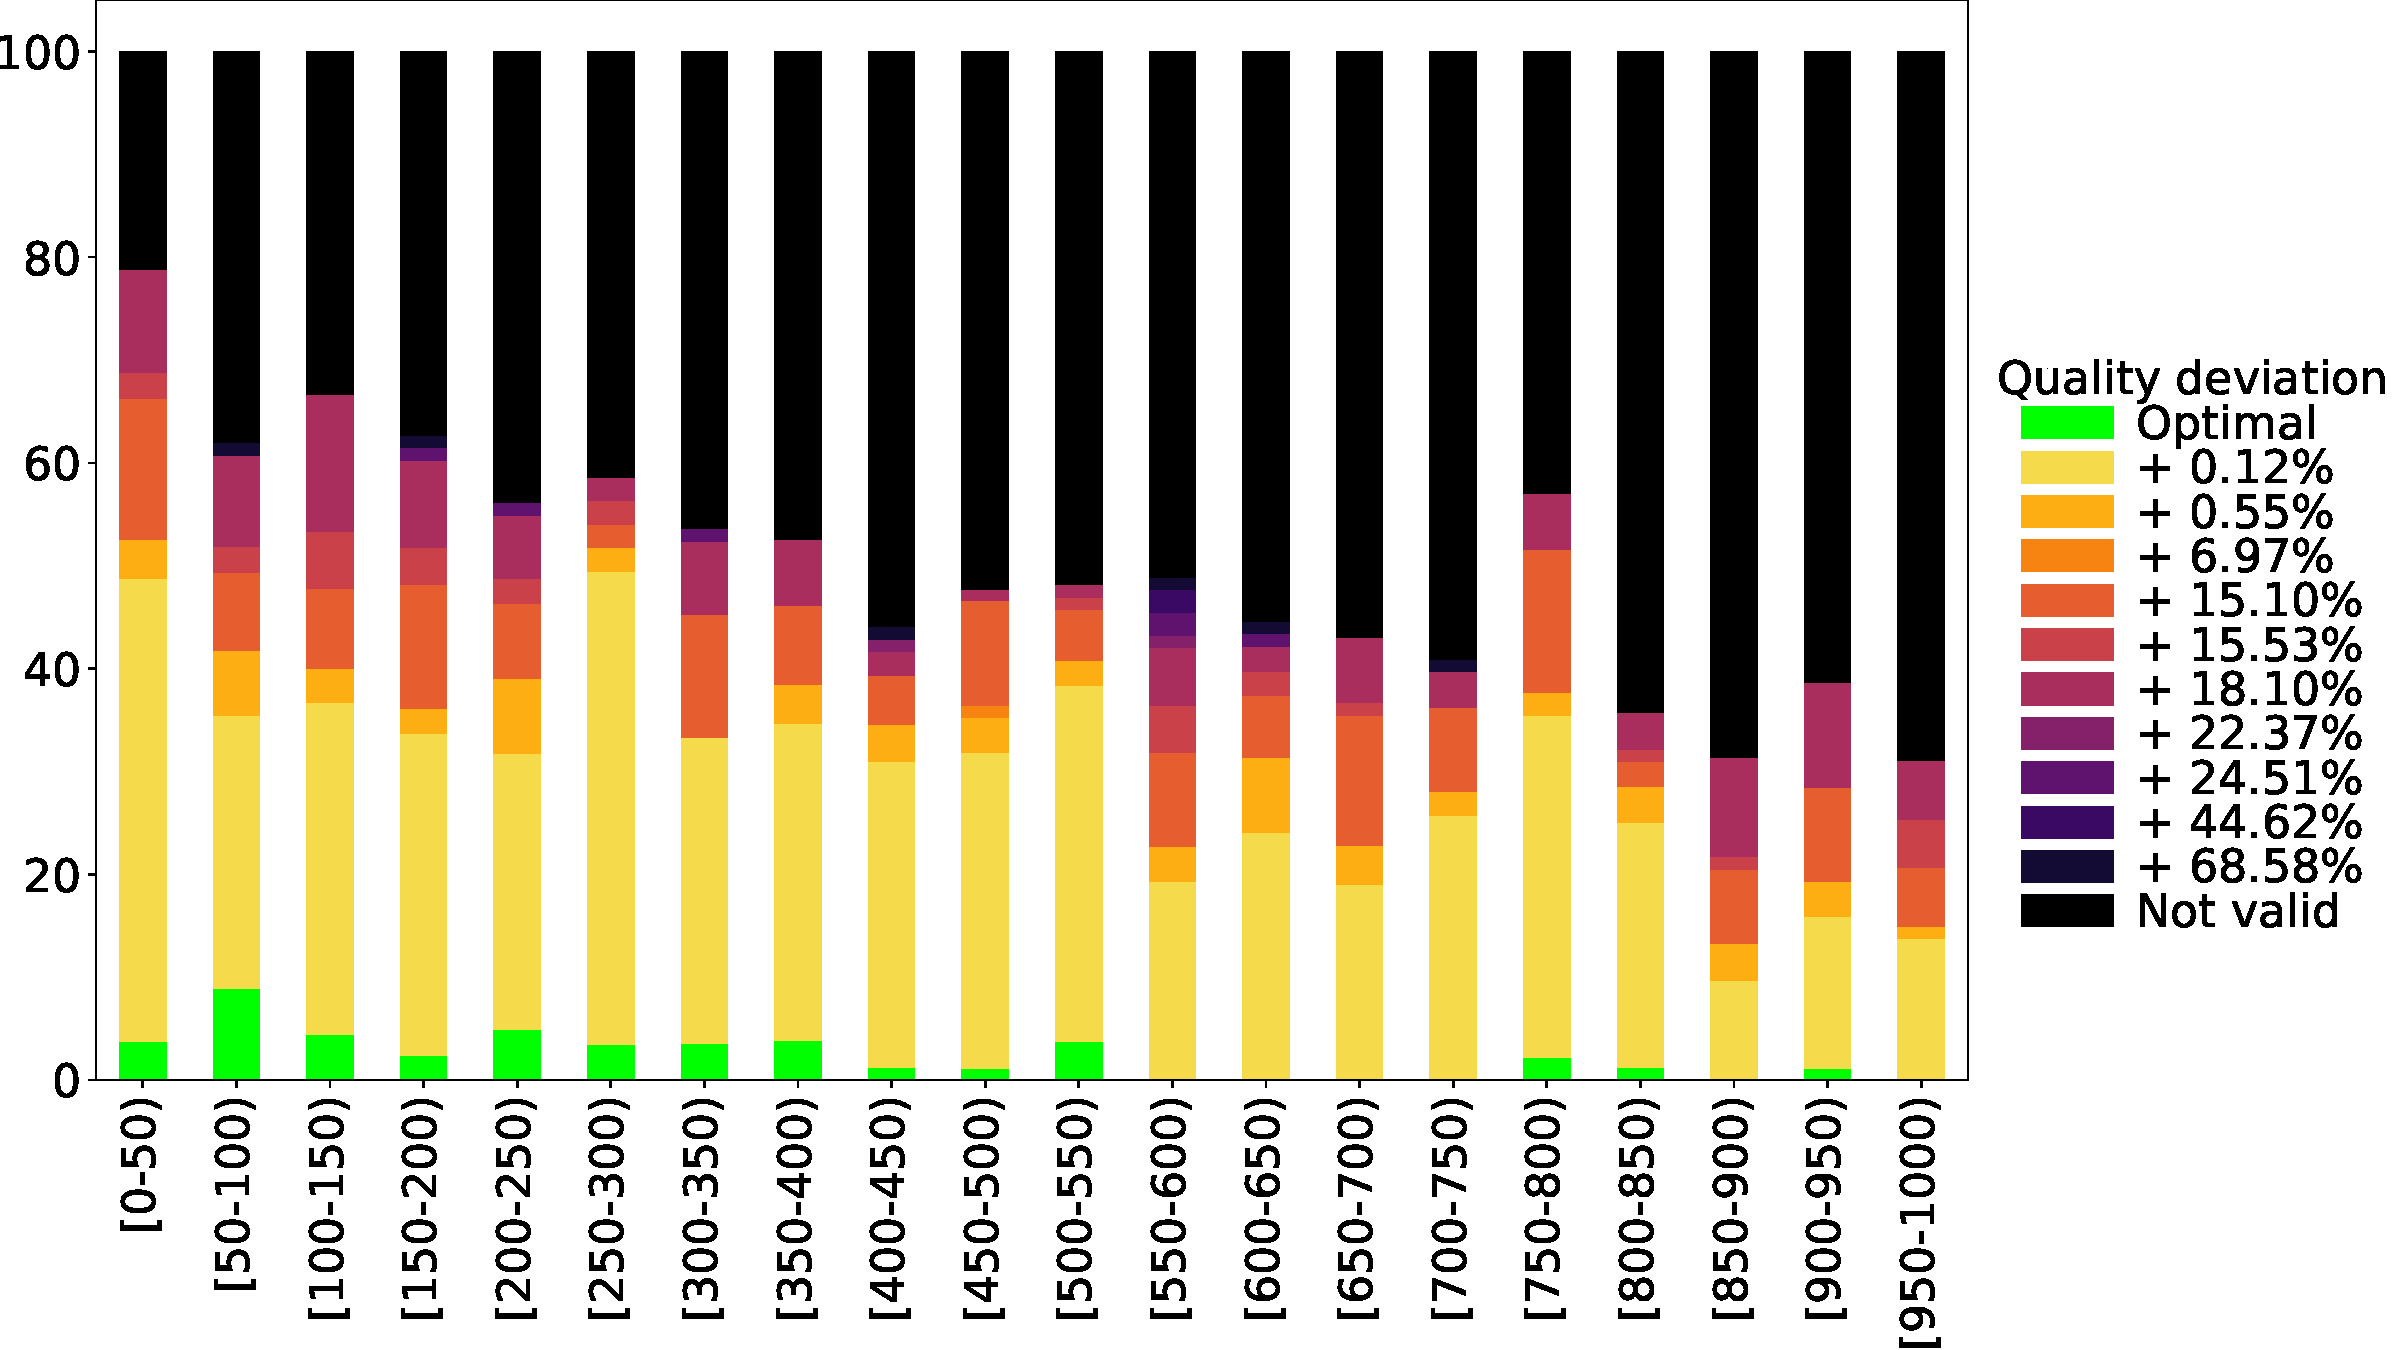
\includegraphics[width=\textwidth]{images/DistrObj/populateSoftwareSolutionAttempts.pdf}
	\caption[populateSoftwareSolutionAttempts parameter values distribution for smaller problem]{populateSoftwareSolutionAttempts parameter values distribution for smaller problem}
	\label{fig:populateSoftwareSolutionAttempts_Obj}
\end{figure}